\chapter[Appendix: Candidate Braids for Track 13]{Appendix: Candidate Braids for Track 13}
\label{app:candidate_braids_track_13}

\section{Summary of Candidate Braid Families}
\label{sec:summary_track13_braids}

Through the exhaustive train track case analysis of Track 13 in the stratum $(2;1^6;3^2)$ (the full details of which are presented in Appendix \ref{app:case_analysis_track13}), we isolate exactly 4 candidate families of train track maps. If the pseudo-Anosov representative $\phi_\Phi$ has no interior fixed points, then its mapping class $\Phi$ must be conjugate to the lift of one of the following 4 braid families.

\vspace{0.3cm}
\begingroup
\raggedbottom
\begin{enumerate}
    \item $\displaystyle \Delta^{2i} \big( \allowbreak\sigma_{4}^{-1}\allowbreak\sigma_{3}\allowbreak\sigma_{2}\allowbreak\sigma_{1}\allowbreak\sigma_{2}^{-1}\allowbreak\sigma_{3}\allowbreak\sigma_{3}\allowbreak\sigma_{2}\allowbreak\sigma_{1}\allowbreak\sigma_{3}\allowbreak\sigma_{2}\allowbreak\sigma_{4}\allowbreak\sigma_{3}\allowbreak\sigma_{4}^{-1}\allowbreak\sigma_{5}^{-1}\allowbreak\sigma_{5}^{-1}\allowbreak\sigma_{4}^{-1}\allowbreak\sigma_{3}^{-1}\allowbreak\sigma_{2}^{-1}\allowbreak\sigma_{1}^{-1}\allowbreak\sigma_{1}^{-1} \cdot L \cdot \Lambda_6 \big)^{-1}$
    \item $\displaystyle \Delta^{2i} \big( \allowbreak\sigma_{4}^{-1}\allowbreak\sigma_{3}\allowbreak\sigma_{2}\allowbreak\sigma_{1}\allowbreak\sigma_{2}^{-1}\allowbreak\sigma_{3}^{-1}\allowbreak\sigma_{1}^{-1}\allowbreak\sigma_{2}^{-1}\allowbreak\sigma_{1}\allowbreak\sigma_{2}\allowbreak\sigma_{3}\allowbreak\sigma_{3}\allowbreak\sigma_{2}\allowbreak\sigma_{1}\allowbreak\sigma_{3}\allowbreak\sigma_{2}\allowbreak\sigma_{4}\allowbreak\sigma_{3}\allowbreak\sigma_{5}^{-1}\allowbreak\sigma_{5}^{-1}\allowbreak\sigma_{4}^{-1}\allowbreak\sigma_{3}^{-1}\allowbreak\sigma_{2}^{-1}\allowbreak\sigma_{1}^{-1}\allowbreak\sigma_{1}^{-1} \cdot L \cdot \Lambda_6 \big)^{-1}$
    \item $\displaystyle \Delta^{2i} \big( \allowbreak\sigma_{4}^{-1}\allowbreak\sigma_{3}\allowbreak\sigma_{2}\allowbreak\sigma_{1}^{-1}\allowbreak\sigma_{3}\allowbreak\sigma_{3}\allowbreak\sigma_{2}\allowbreak\sigma_{1}\allowbreak\sigma_{3}\allowbreak\sigma_{2}\allowbreak\sigma_{4}\allowbreak\sigma_{3}\allowbreak\sigma_{5}^{-1}\allowbreak\sigma_{1}\allowbreak\sigma_{2}\allowbreak\sigma_{3}\allowbreak\sigma_{2}\allowbreak\sigma_{1}\allowbreak\sigma_{4}\allowbreak\sigma_{3}\allowbreak\sigma_{2}\allowbreak\sigma_{4}\allowbreak\sigma_{3}\allowbreak\sigma_{5}\allowbreak\sigma_{4}\allowbreak\sigma_{5}\allowbreak\sigma_{5} \big)^{-1}$
    \item $\displaystyle \Delta^{2i} \big( \allowbreak\sigma_{4}\allowbreak\sigma_{2}\allowbreak\sigma_{3}\allowbreak\sigma_{4}^{-1}\allowbreak\sigma_{5}^{-1}\allowbreak\sigma_{4}^{-1}\allowbreak\sigma_{5}^{-1}\allowbreak\sigma_{3}^{-1}\allowbreak\sigma_{4}^{-1}\allowbreak\sigma_{2}\allowbreak\sigma_{3}^{-1}\allowbreak\sigma_{2}^{-1}\allowbreak\sigma_{1}^{-1}\allowbreak\sigma_{1}^{-1} \cdot L \cdot \Lambda_6 \big)^{-1}$
\end{enumerate}
\endgroup

\clearpage

\section{Base Braids \texorpdfstring{$\Lambda_6$}{Lambda\_6} and \texorpdfstring{$L$}{L}}
Before we list the braids carrying candidate train track maps for Track 13, we introduce the following base braids, which we will call $\Lambda_6$ and $L$:

\begin{flushleft}
$\displaystyle \Lambda_6 = \allowbreak\sigma_{1}\allowbreak\sigma_{2}\allowbreak\sigma_{1}\allowbreak\sigma_{3}\allowbreak\sigma_{2}\allowbreak\sigma_{1}\allowbreak\sigma_{4}\allowbreak\sigma_{3}\allowbreak\sigma_{2}\allowbreak\sigma_{1}\allowbreak\sigma_{5}\allowbreak\sigma_{4}\allowbreak\sigma_{3}\allowbreak\sigma_{2}\allowbreak\sigma_{1}$
\end{flushleft}

\begin{flushleft}
$\displaystyle L = \allowbreak\sigma_{1}^{-1}\allowbreak\sigma_{5}\allowbreak\sigma_{4}\allowbreak\sigma_{3}\allowbreak\sigma_{5}\allowbreak\sigma_{4}\allowbreak\sigma_{5}$
\end{flushleft}

We shall make use of $\Lambda_6$ and $L$ occasionally in constructing candidate braids for Track 13.

\clearpage

\section{Candidate Family 1 (Chirk)}\label{sec:track13_chirk}
Train Track Map Candidate Family 1 of Track 13 is shown in Figure \ref{fig:track13_braid_b13_1_map}. See \ref{Chirk} for details.

\begin{figure*}[ht]
    \centering
    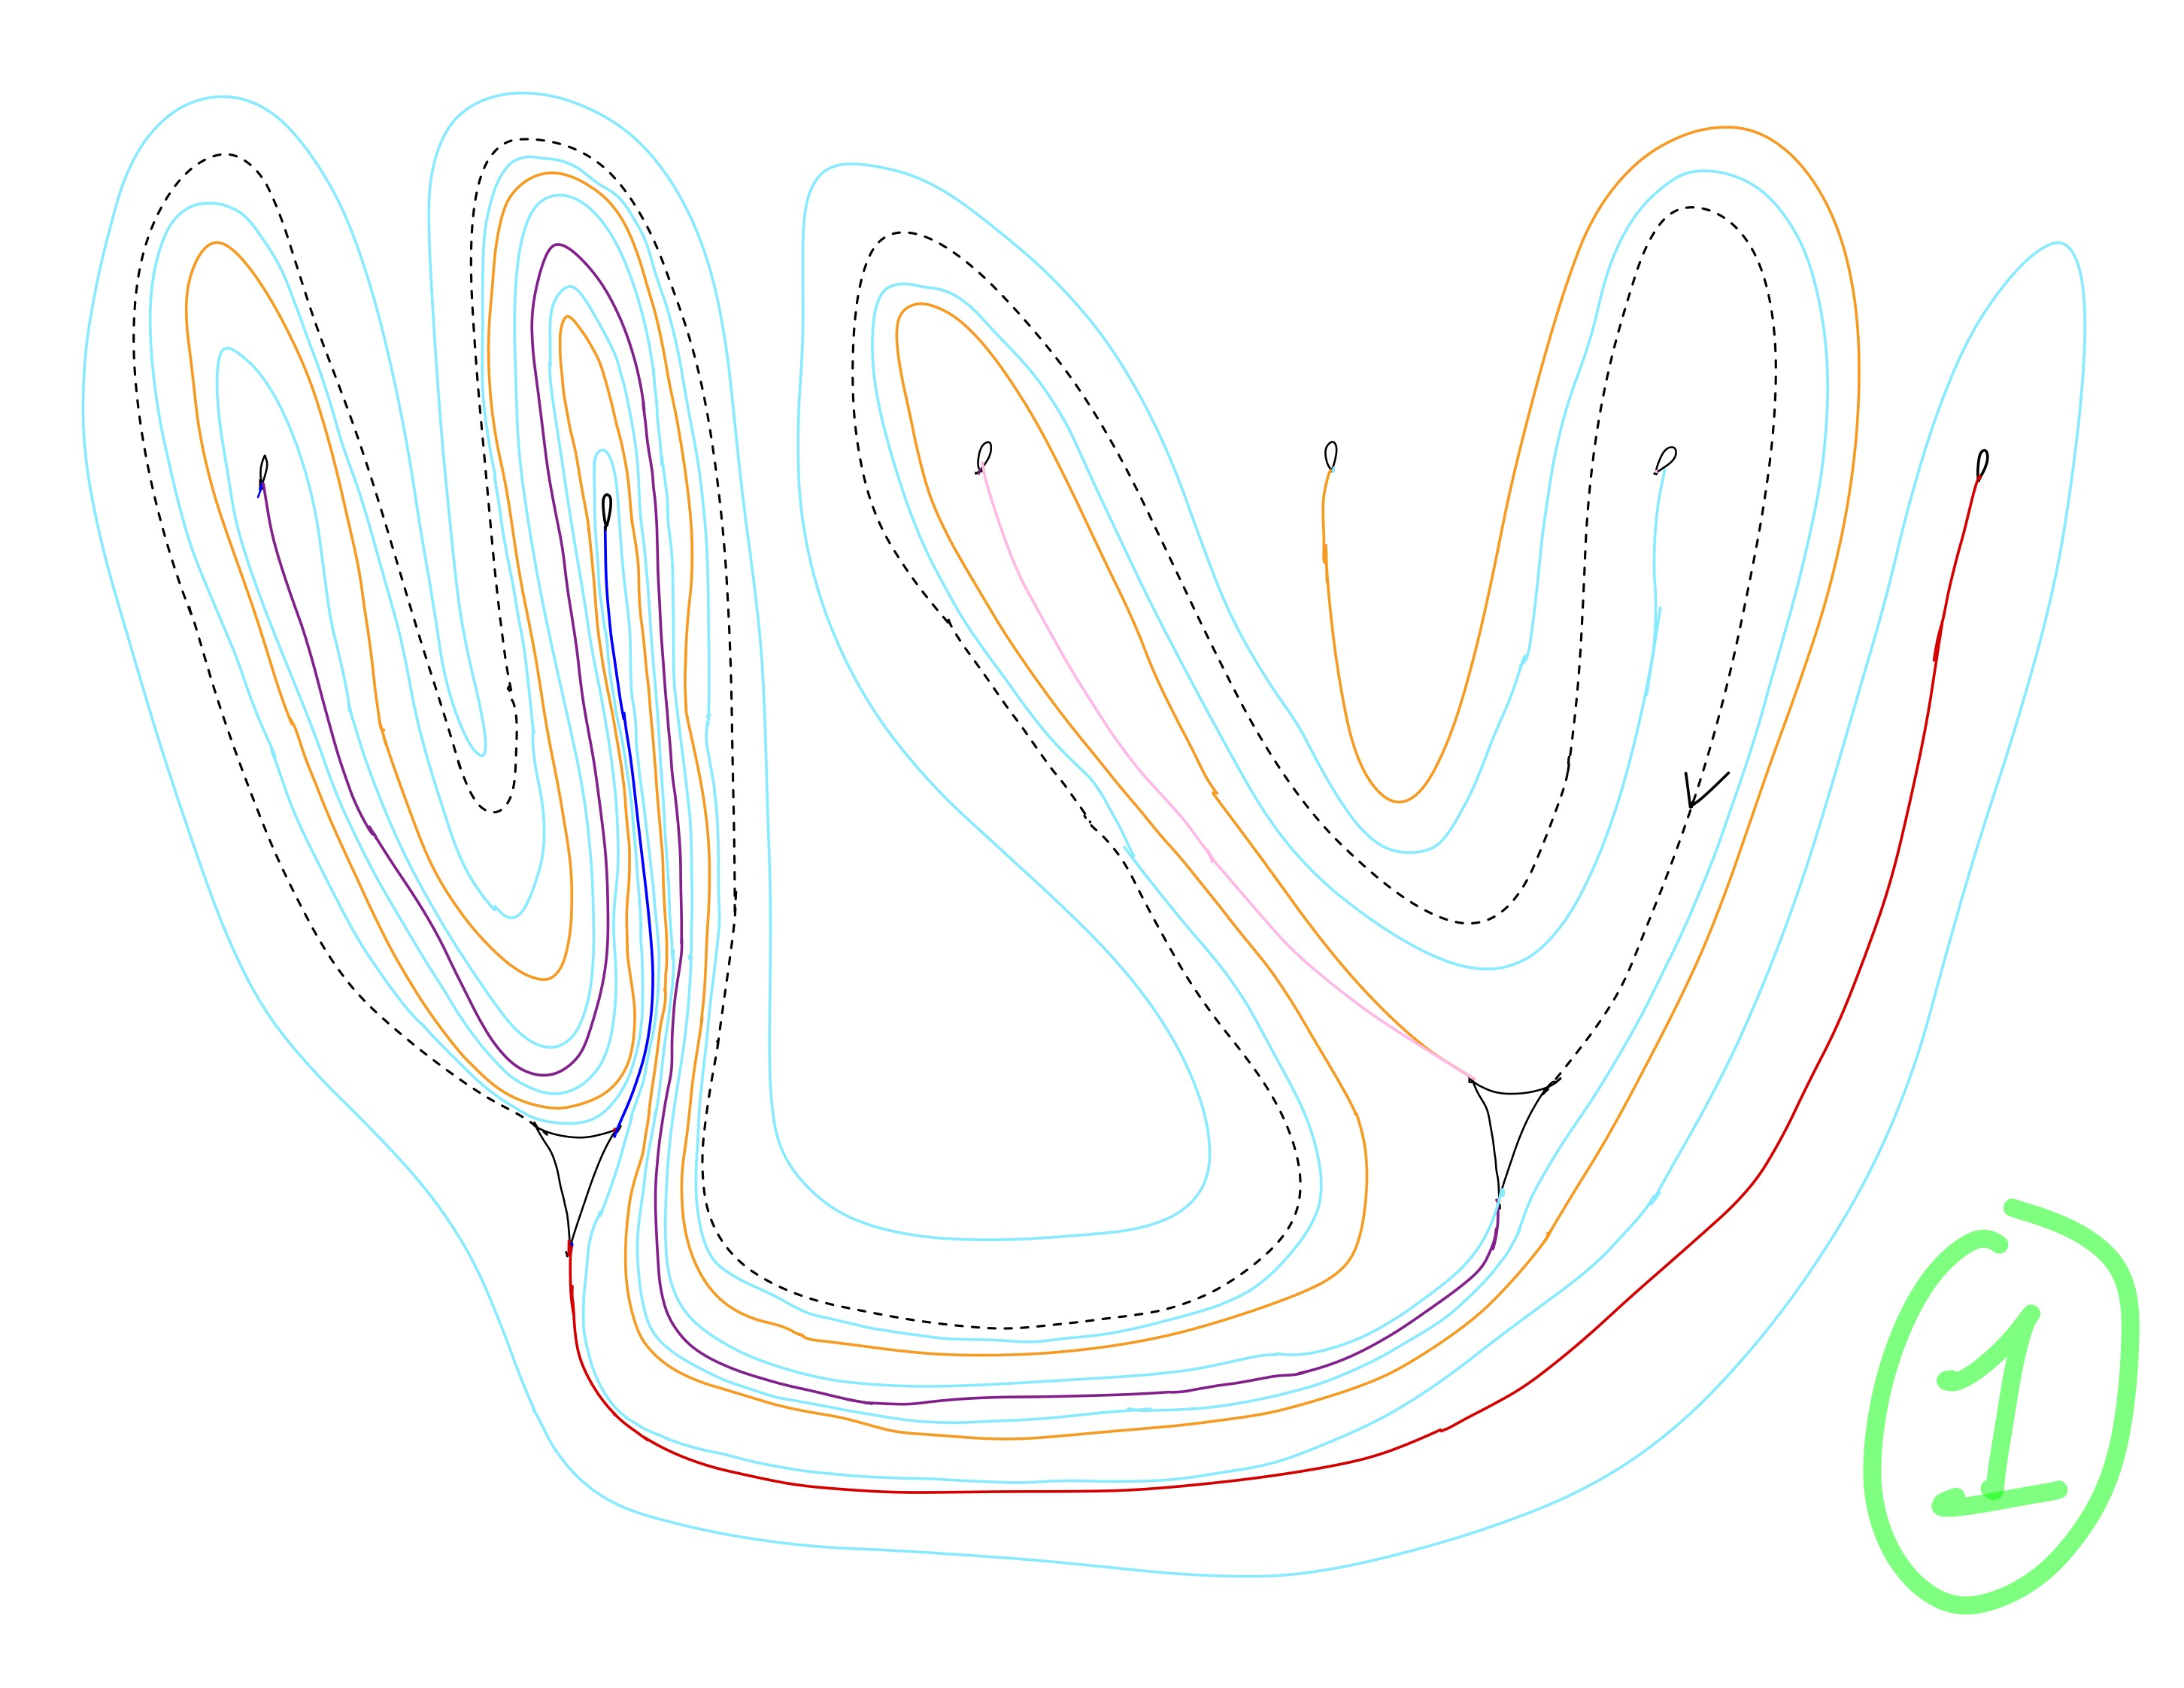
\includegraphics[width=\linewidth, height=0.45\textheight, keepaspectratio]{figures_braid/figures_track_13/Track 13 Braid 1 Chirk-1.jpg}
    \caption{Train Track Map Candidate Family 1 (Chirk) of Track 13.}
    \label{fig:track13_braid_b13_1_map}
\end{figure*}

The inverse of the following braid carries this family of train track maps:
\[
b_1^{13} = \sigma_{4}^{-1} \sigma_{3} \sigma_{2} \sigma_{1} \sigma_{2}^{-1} \sigma_{3} \sigma_{3} \sigma_{2} \sigma_{1} \sigma_{3} \sigma_{2} \sigma_{4} \sigma_{3} \sigma_{4}^{-1} \sigma_{5}^{-1} \sigma_{5}^{-1} \sigma_{4}^{-1} \sigma_{3}^{-1} \sigma_{2}^{-1} \sigma_{1}^{-1} \sigma_{1}^{-1} \circ L \circ \Lambda_6
\]

This is shown in Figure \ref{fig:track13_braid_b13_1}.

\begin{figure*}[p]
    \centering
    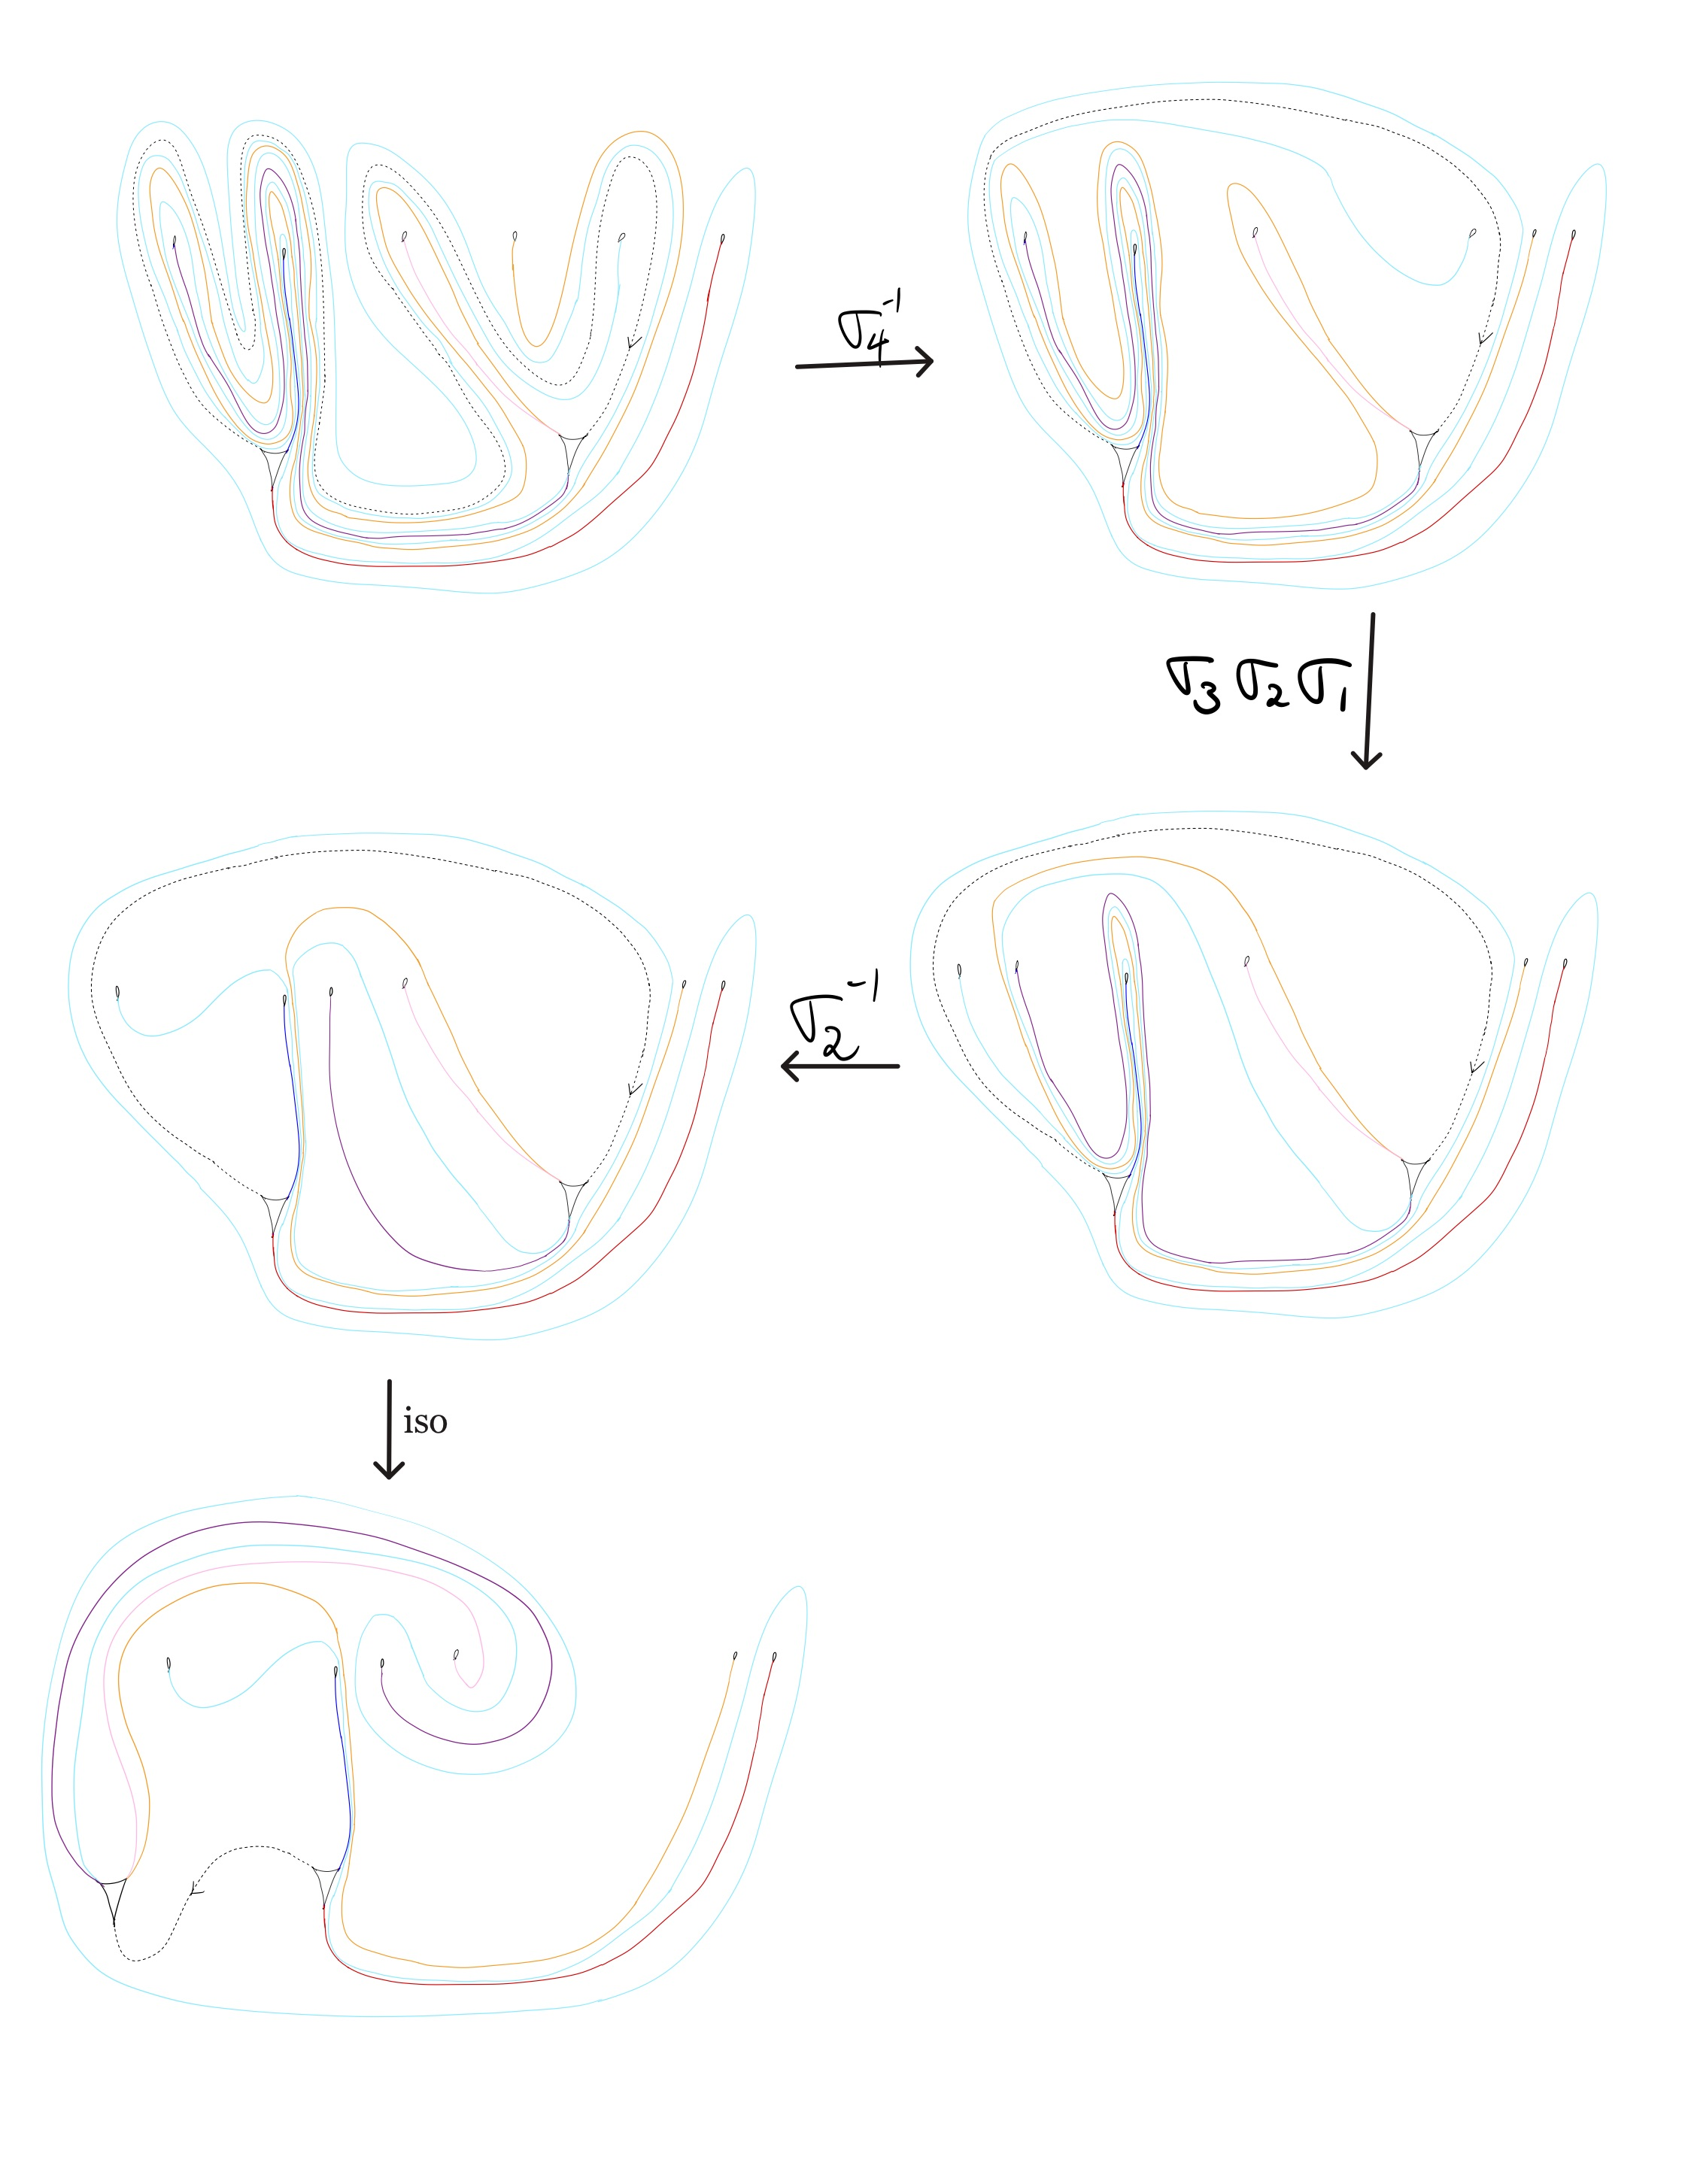
\includegraphics[width=\linewidth, height=0.45\textheight, keepaspectratio]{figures_braid/figures_track_13/Track 13 Braid 1 Chirk-2.jpg}%
    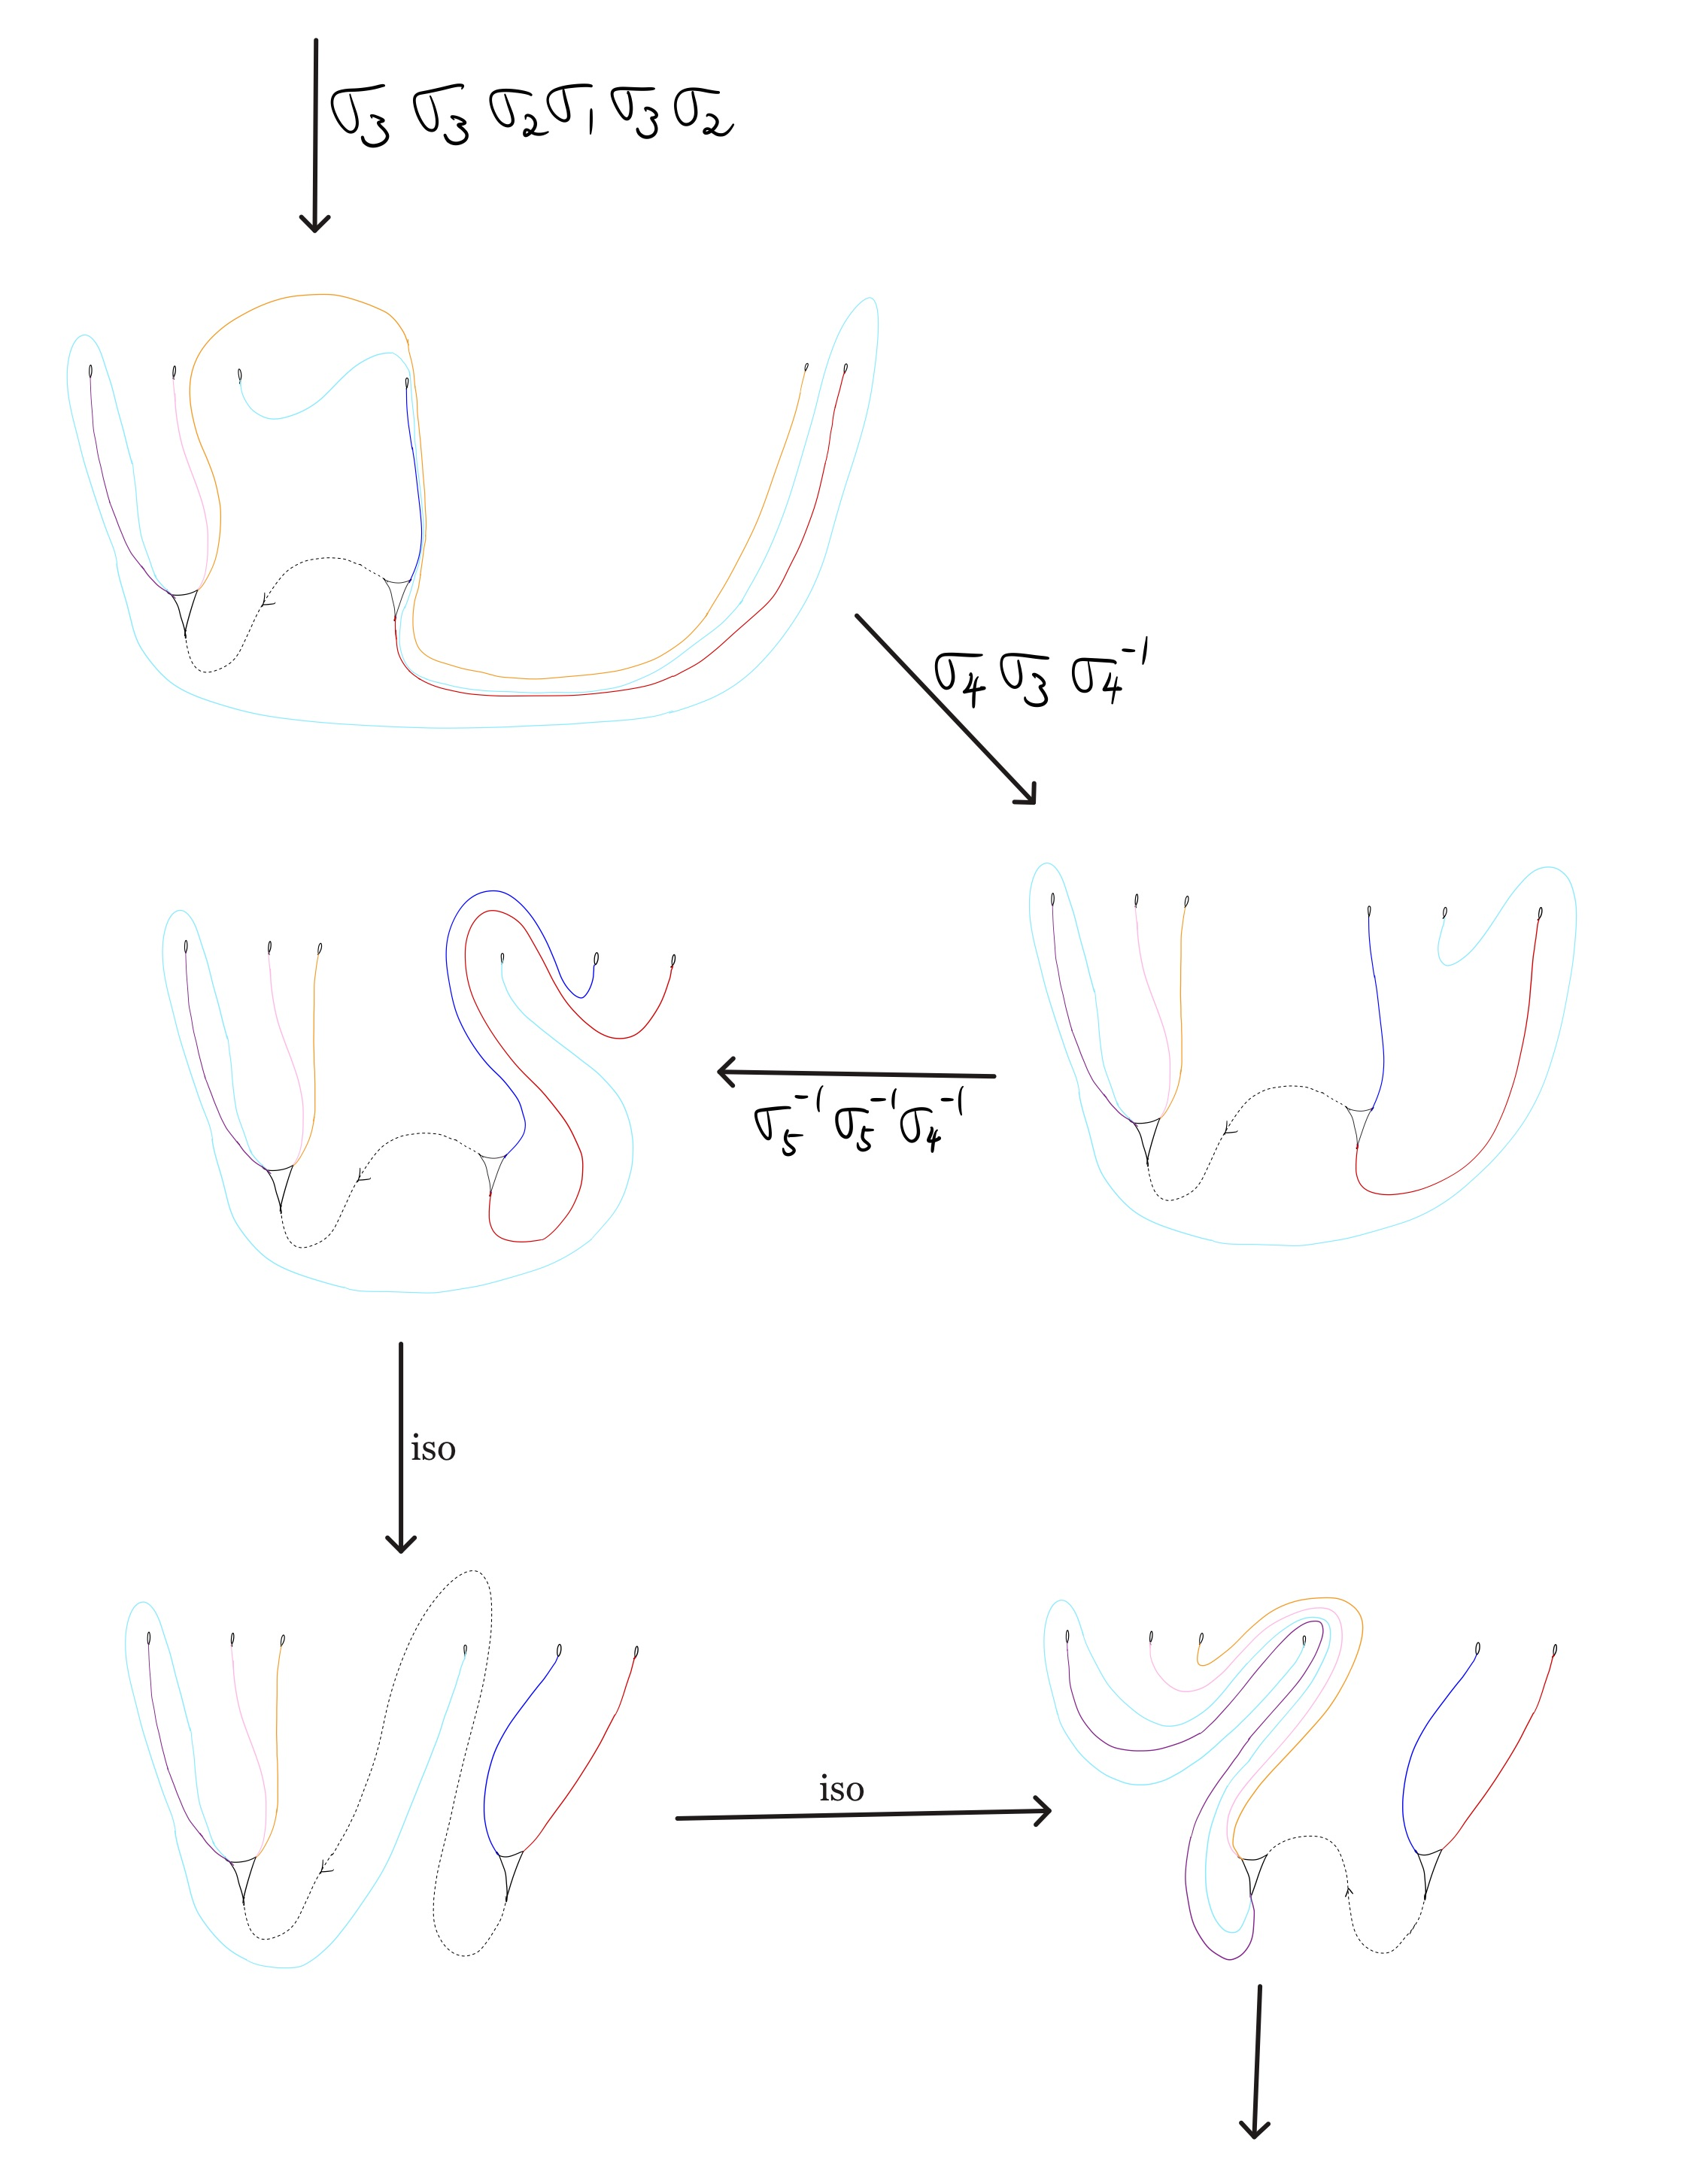
\includegraphics[width=\linewidth, height=0.45\textheight, keepaspectratio]{figures_braid/figures_track_13/Track 13 Braid 1 Chirk-3.jpg}
    \caption{This sequence shows the inverse of the braid $b_1^{13}$ carries Train Track Candidate Family 1.}
    \label{fig:track13_braid_b13_1}
\end{figure*}

\clearpage

\section{Candidate Family 2 (Cagmag)}\label{sec:track13_cagmag}
Train Track Map Candidate Family 2 of Track 13 is shown in Figure \ref{fig:track13_braid_b13_2_map}. See \ref{Cagmag} for details.

\begin{figure*}[ht]
    \centering
    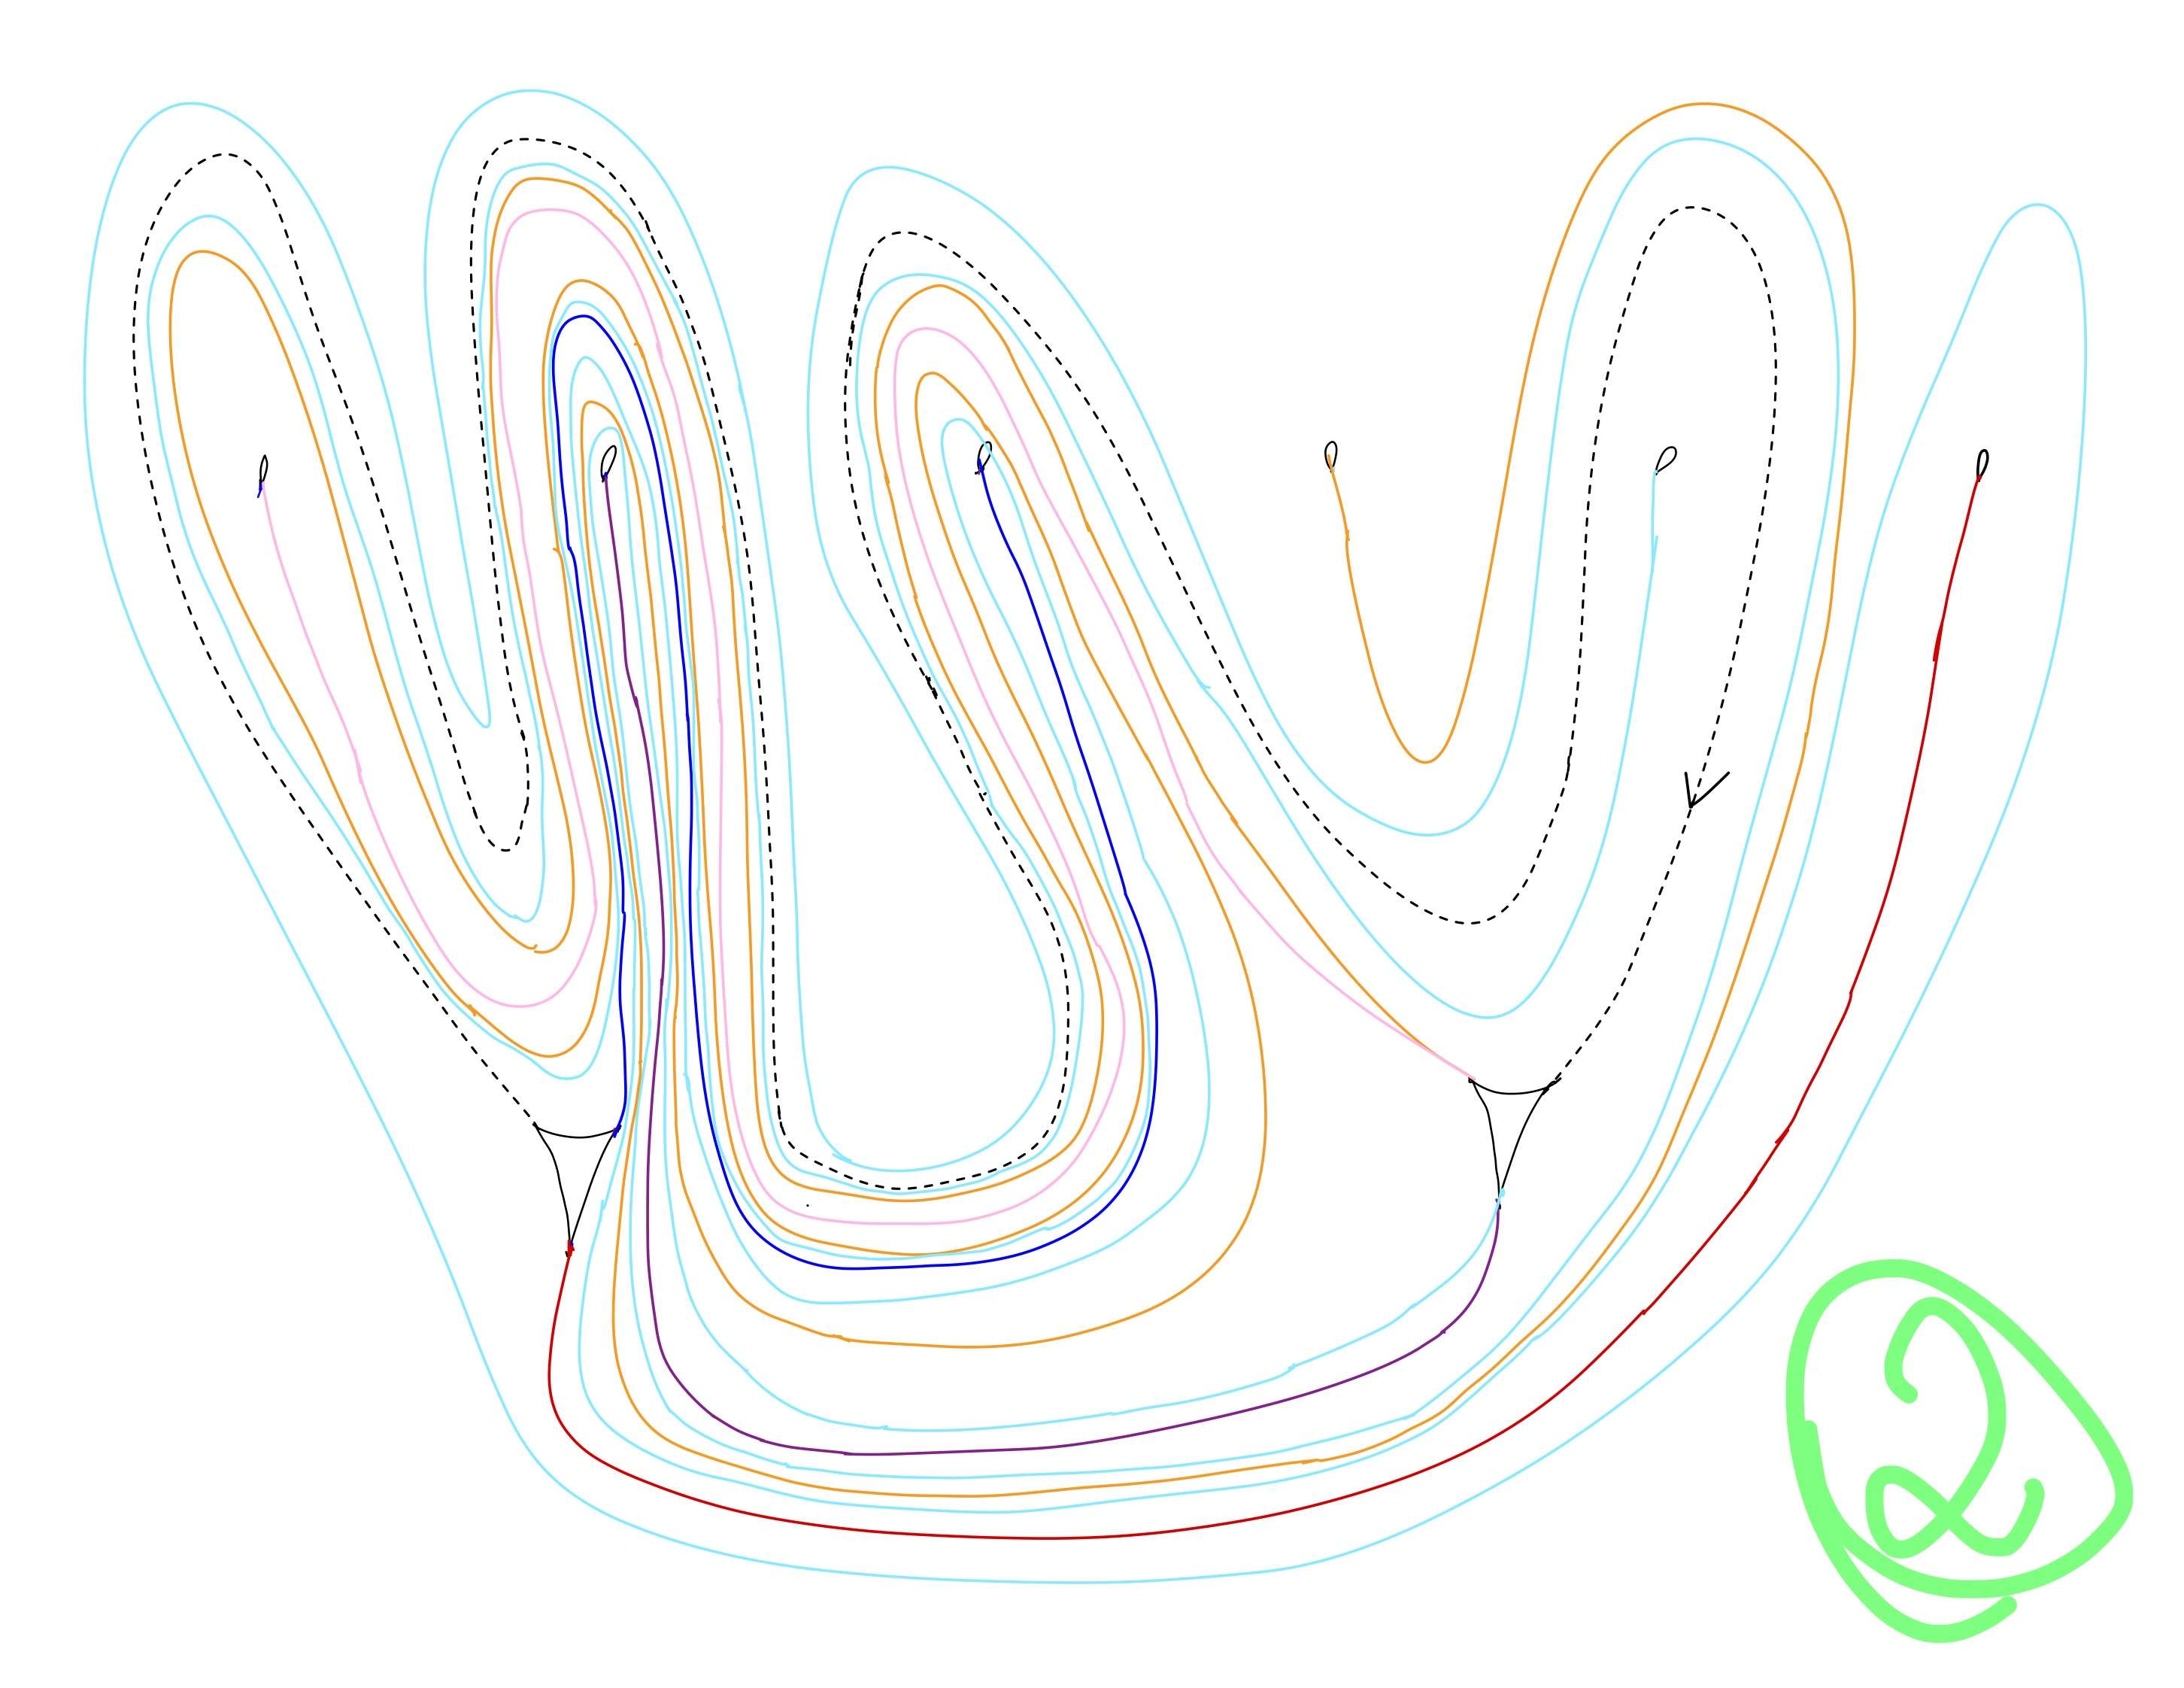
\includegraphics[width=\linewidth, height=0.45\textheight, keepaspectratio]{figures_braid/figures_track_13/Track 13 Braid 2 Cagmag-1.jpg}
    \caption{Train Track Map Candidate Family 2 (Cagmag) of Track 13.}
    \label{fig:track13_braid_b13_2_map}
\end{figure*}

The inverse of the following braid carries this family of train track maps:
\[
b_2^{13} = \sigma_{4}^{-1} \sigma_{3} \sigma_{2} \sigma_{1} \sigma_{2}^{-1} \sigma_{3}^{-1} \sigma_{1}^{-1} \sigma_{2}^{-1} \sigma_{1} \sigma_{2} \sigma_{3} \sigma_{3} \sigma_{2} \sigma_{1} \sigma_{3} \sigma_{2} \sigma_{4} \sigma_{3} \sigma_{5}^{-1} \sigma_{5}^{-1} \sigma_{4}^{-1} \sigma_{3}^{-1} \sigma_{2}^{-1} \sigma_{1}^{-1} \sigma_{1}^{-1} \circ L \circ \Lambda_6
\]

This is shown in Figure \ref{fig:track13_braid_b13_2}.

\begin{figure*}[p]
    \centering
    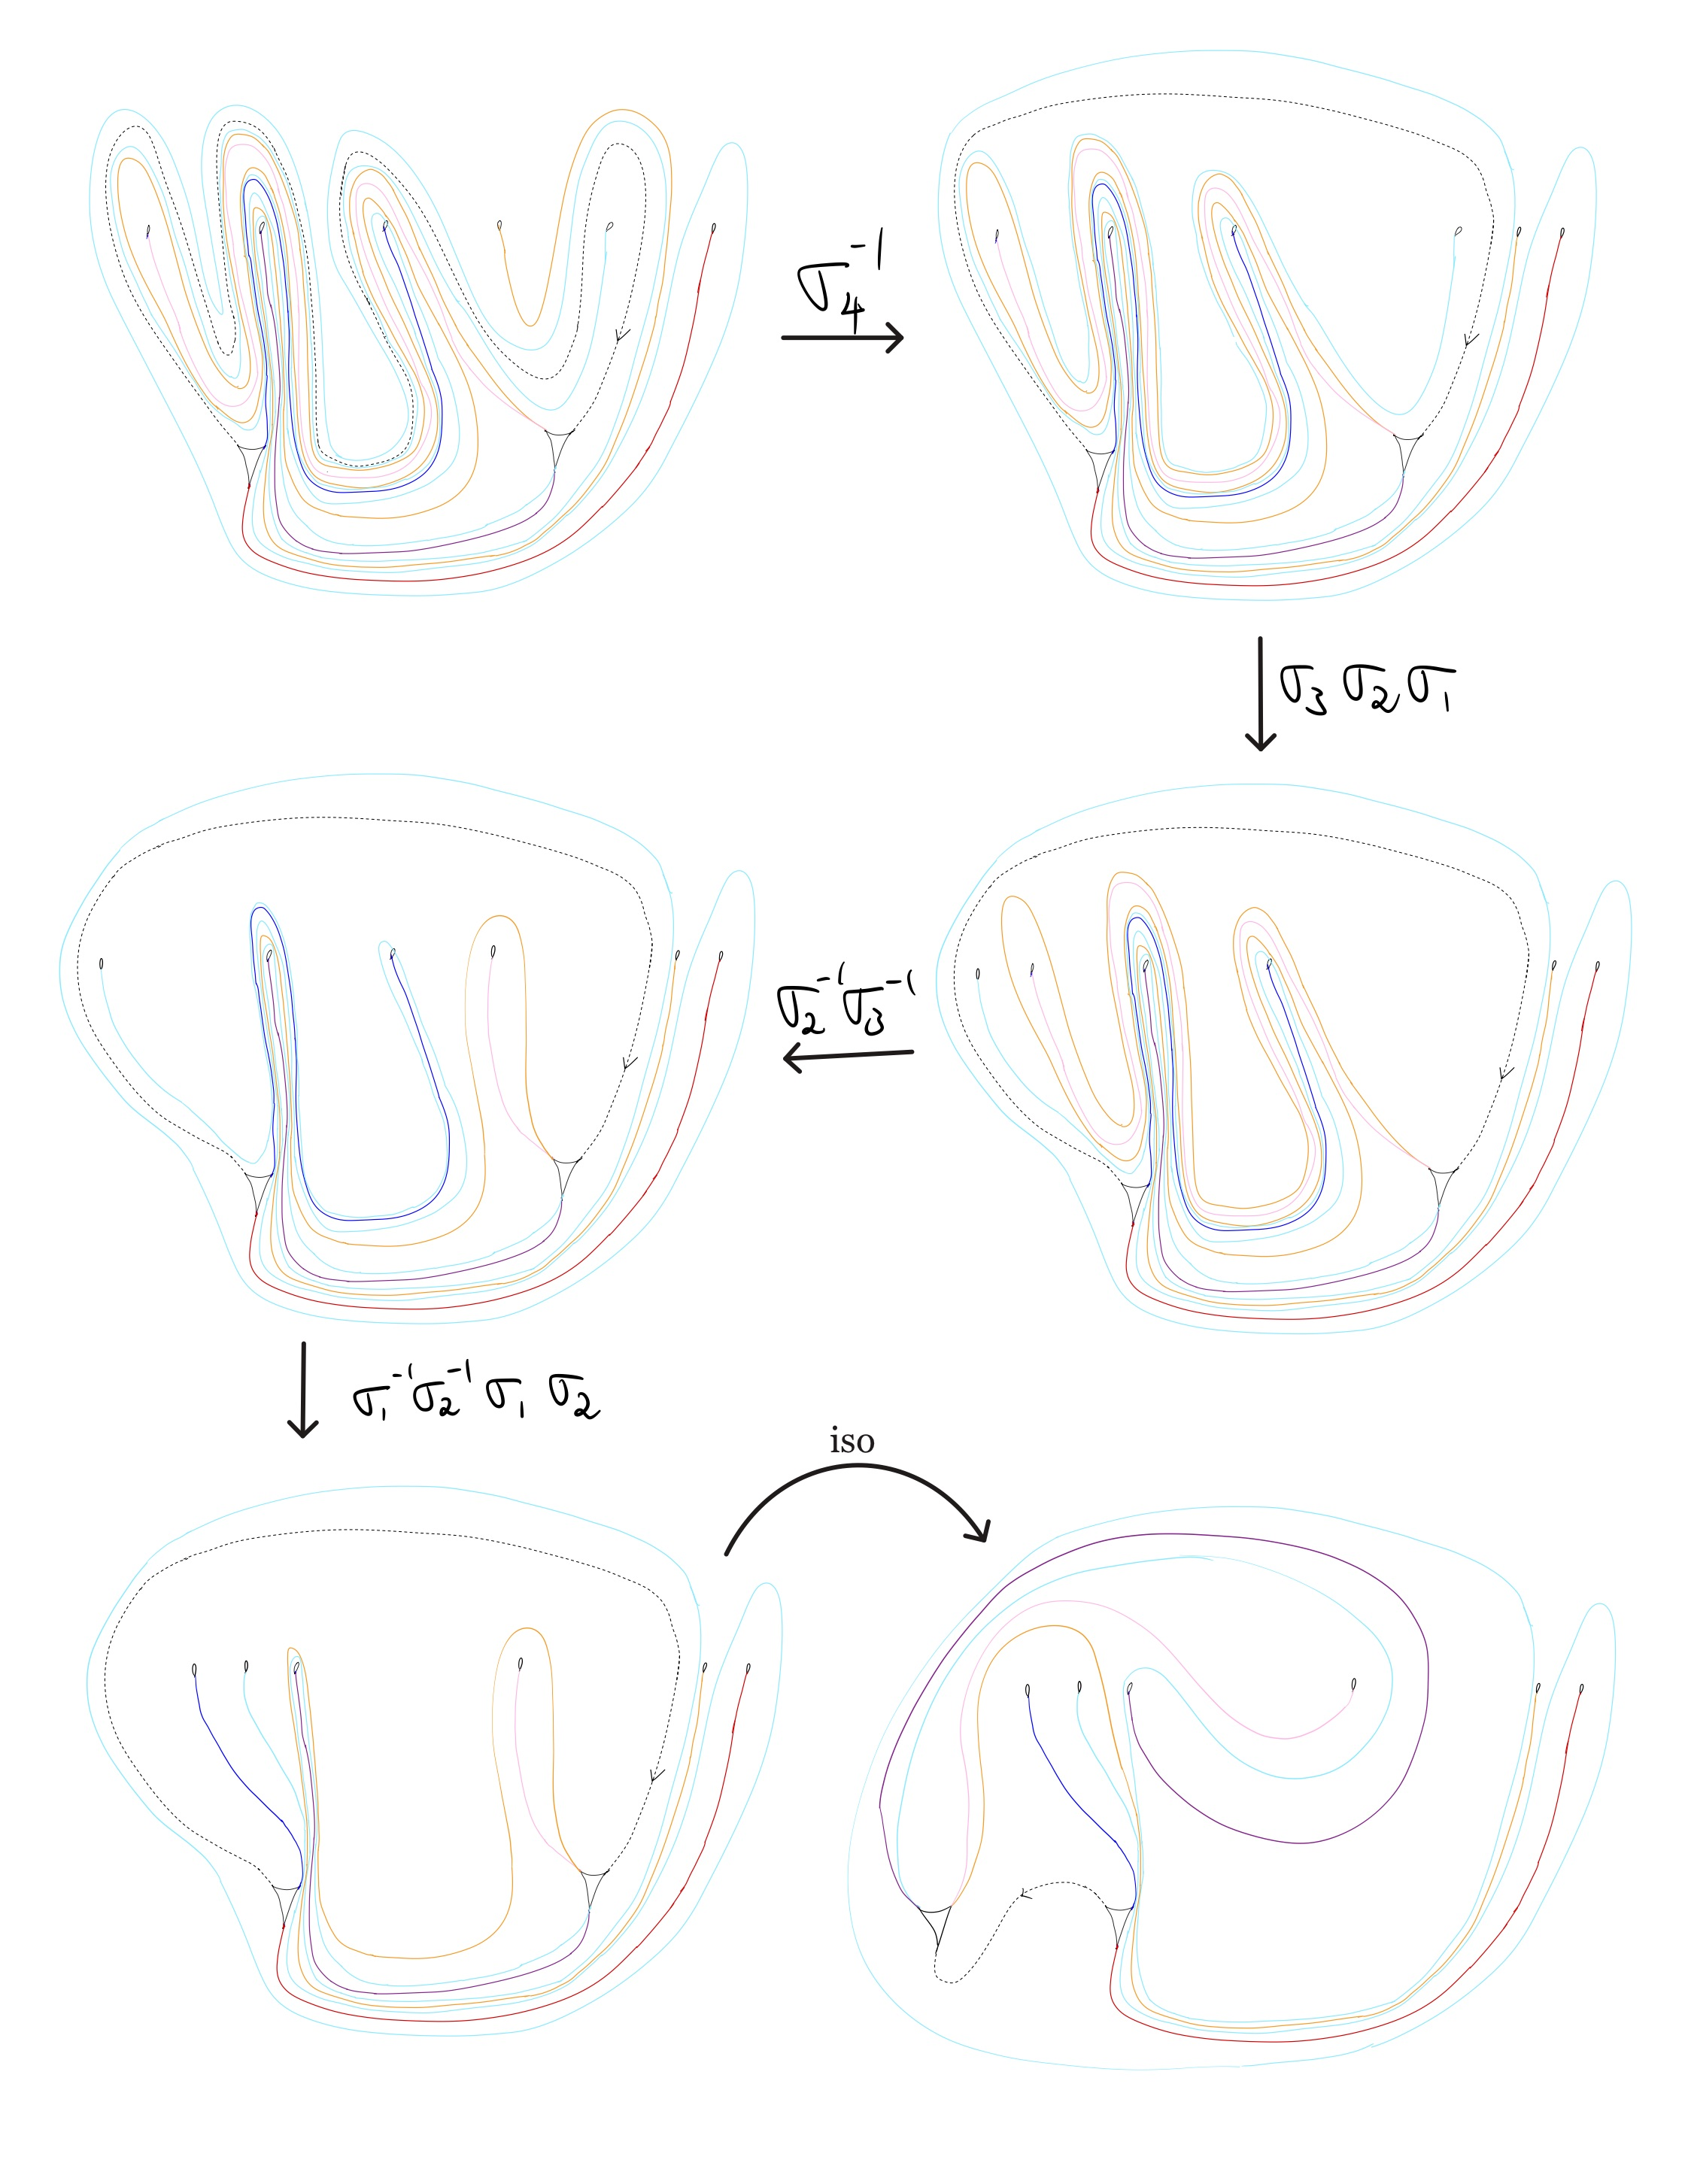
\includegraphics[width=\linewidth, height=0.45\textheight, keepaspectratio]{figures_braid/figures_track_13/Track 13 Braid 2 Cagmag-2.jpg}%
    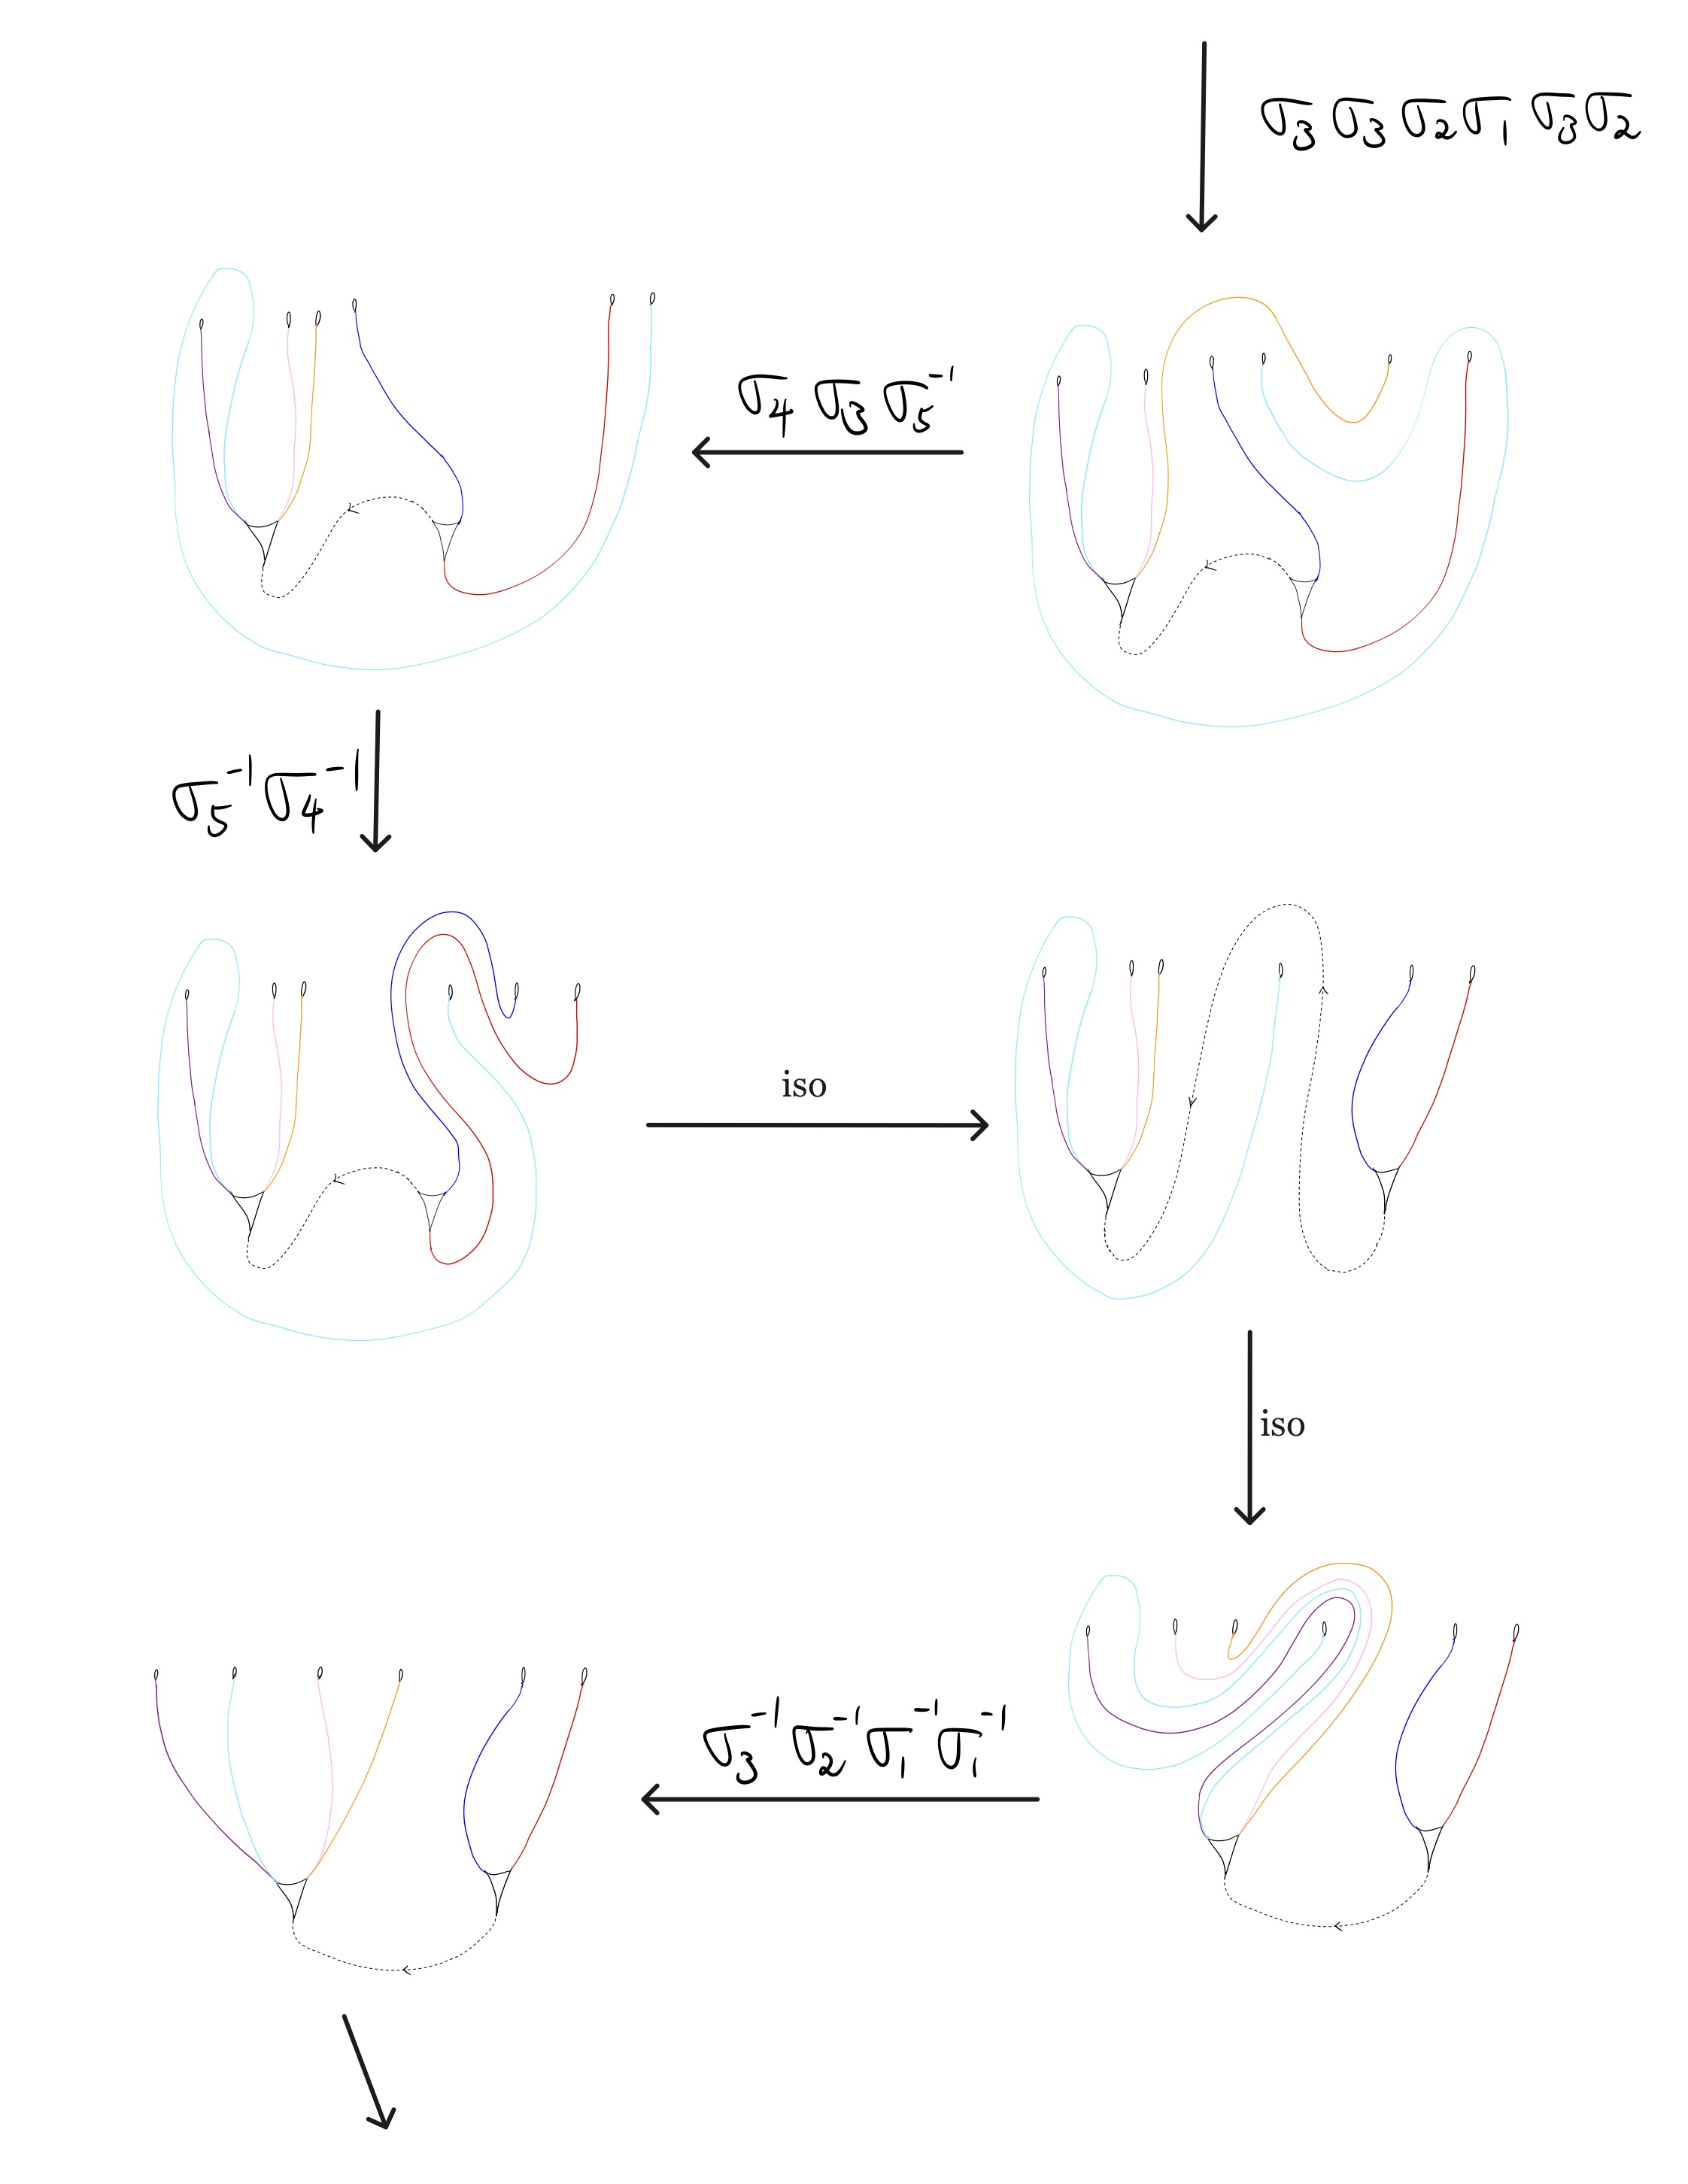
\includegraphics[width=\linewidth, height=0.45\textheight, keepaspectratio]{figures_braid/figures_track_13/Track 13 Braid 2 Cagmag-3.jpg}
    \caption{This sequence shows the inverse of the braid $b_2^{13}$ carries Train Track Candidate Family 2.}
    \label{fig:track13_braid_b13_2}
\end{figure*}

\clearpage

\section{Candidate Family 3 (Boofus)}\label{sec:track13_boofus}
Train Track Map Candidate Family 3 of Track 13 is shown in Figure \ref{fig:track13_braid_b13_3_map}. See \ref{Boofus} for details.

\begin{figure*}[ht]
    \centering
    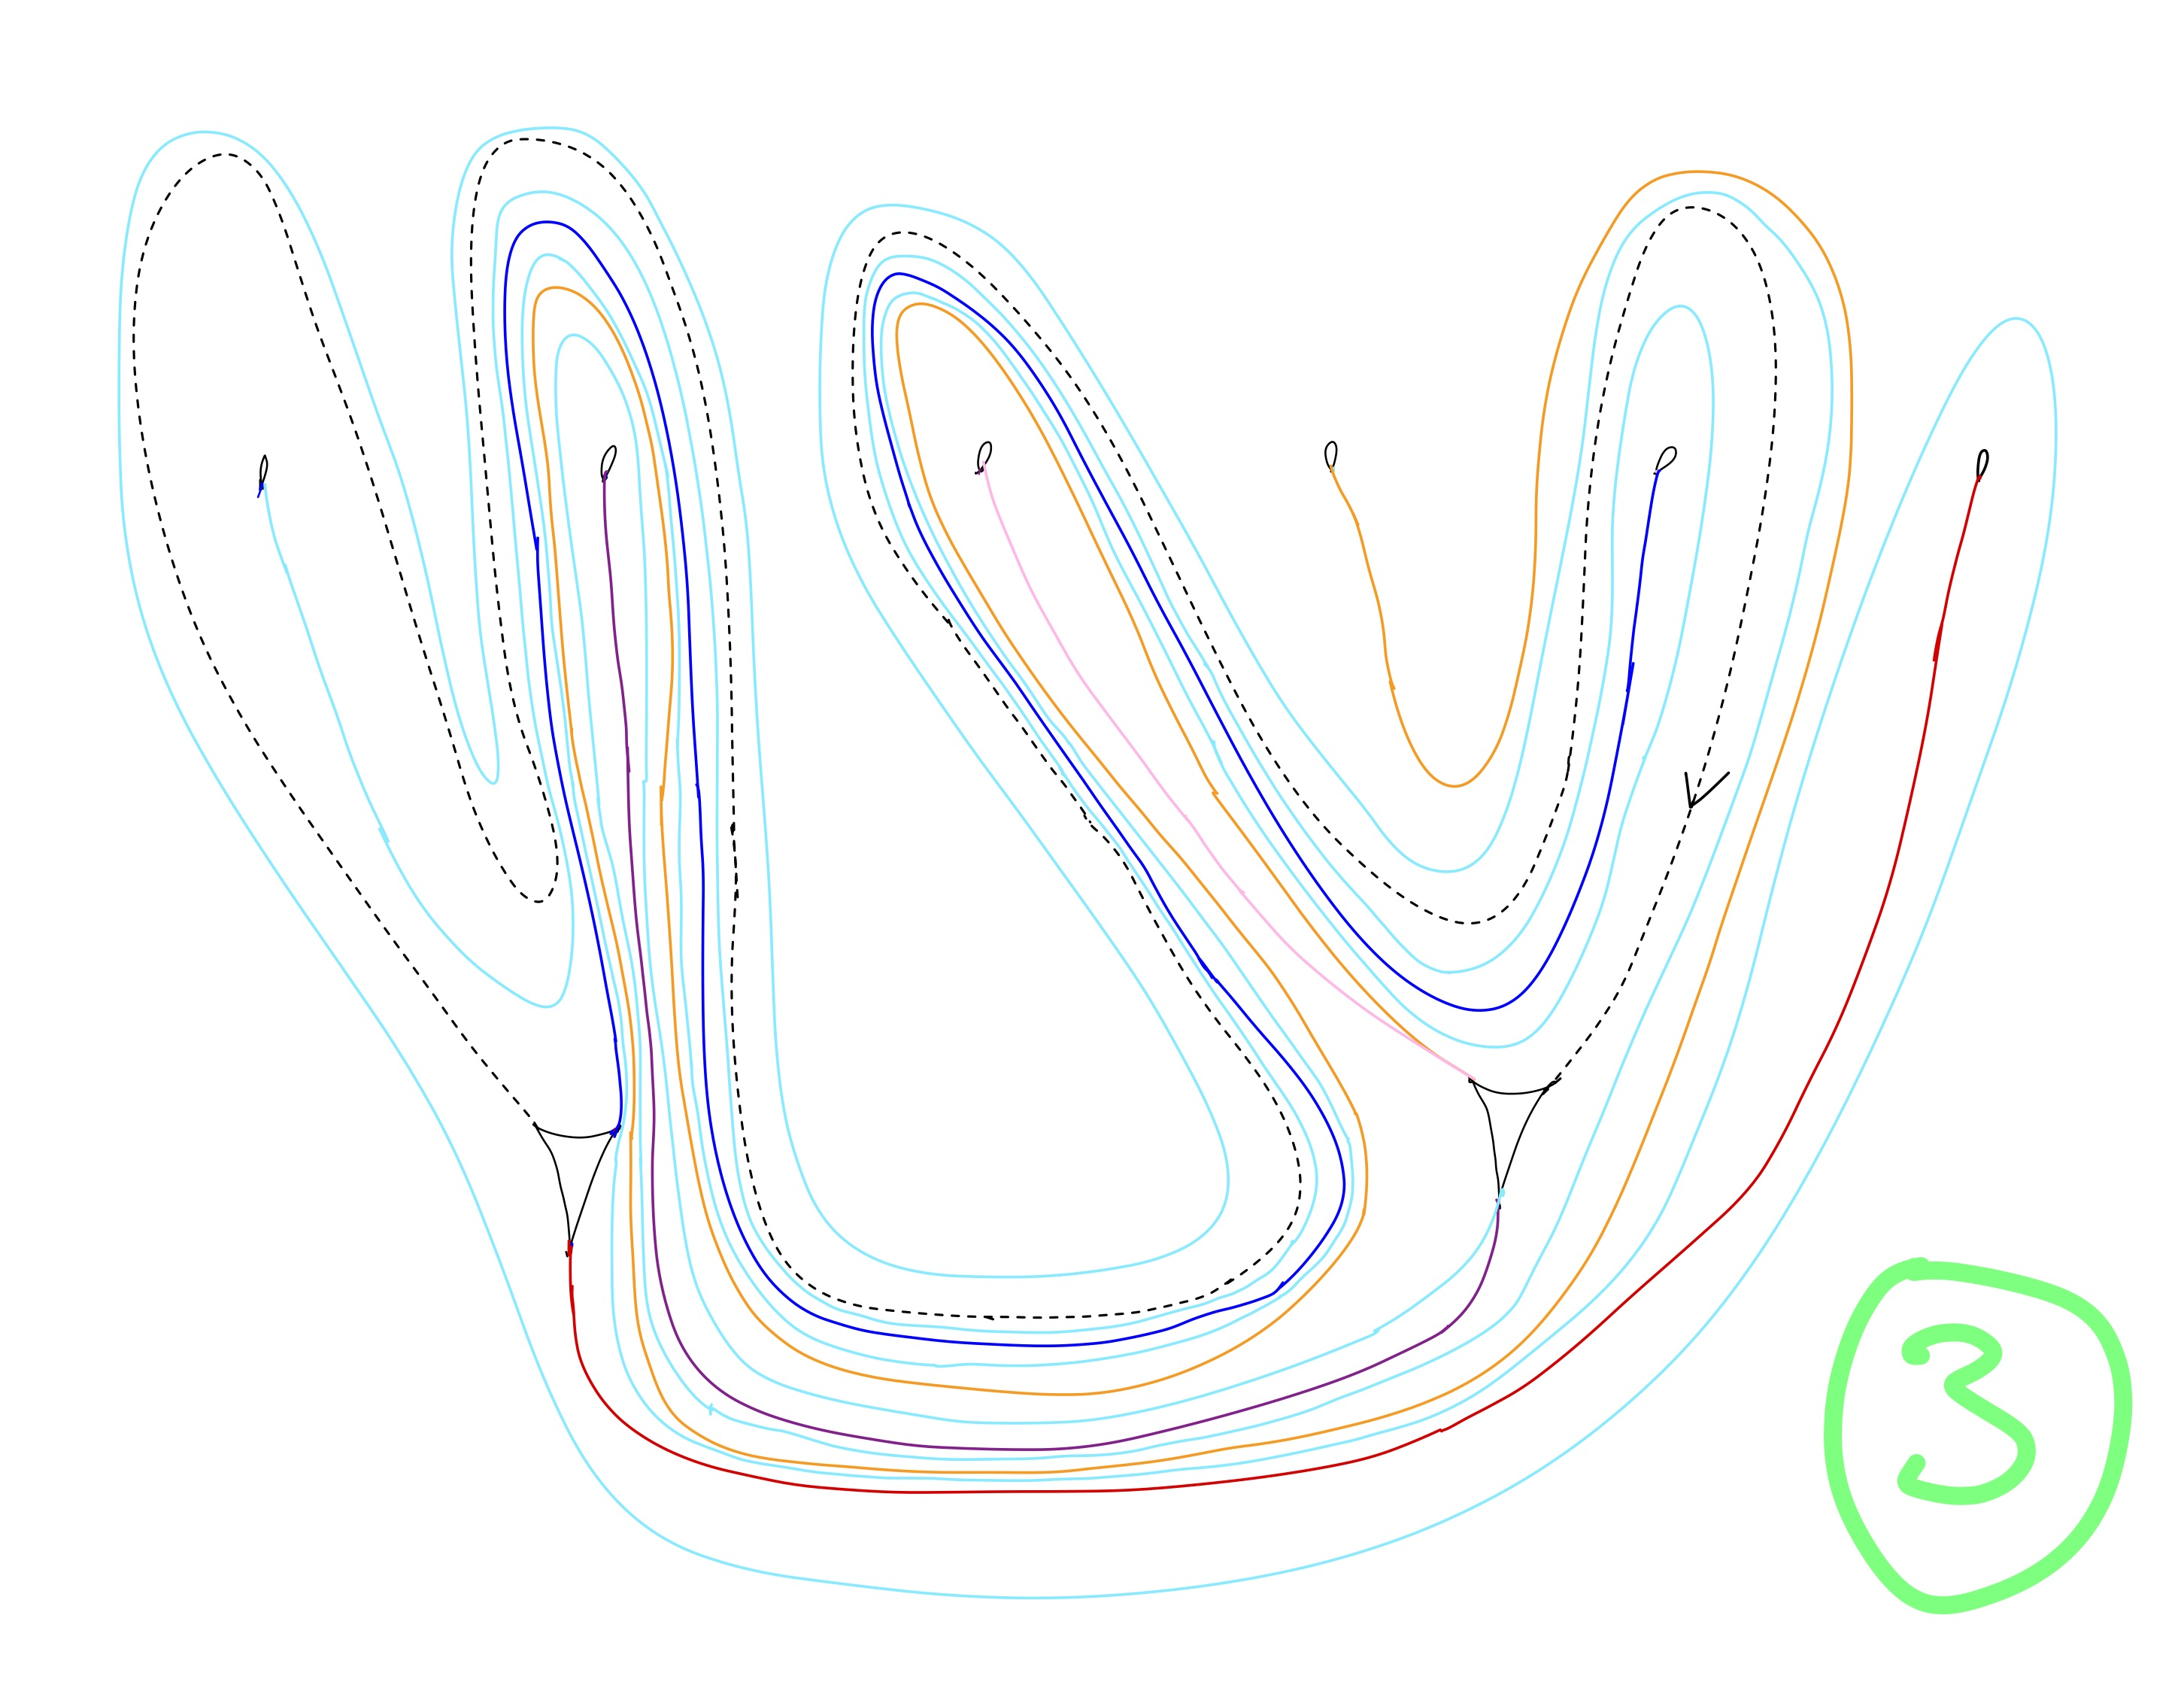
\includegraphics[width=\linewidth, height=0.45\textheight, keepaspectratio]{figures_braid/figures_track_13/Track 13 Braid 3 Boofus-1.jpg}
    \caption{Train Track Map Candidate Family 3 (Boofus) of Track 13.}
    \label{fig:track13_braid_b13_3_map}
\end{figure*}

The inverse of the following braid carries this family of train track maps:
\[
b_3^{13} = \sigma_{4}^{-1} \sigma_{3} \sigma_{2} \sigma_{1}^{-1} \sigma_{3} \sigma_{3} \sigma_{2} \sigma_{1} \sigma_{3} \sigma_{2} \sigma_{4} \sigma_{3} \sigma_{5}^{-1} \sigma_{1} \sigma_{2} \sigma_{3} \sigma_{2} \sigma_{1} \sigma_{4} \sigma_{3} \sigma_{2} \sigma_{4} \sigma_{3} \sigma_{5} \sigma_{4} \sigma_{5} \sigma_{5}
\]

This is shown in Figure \ref{fig:track13_braid_b13_3}.

\begin{figure*}[p]
    \centering
    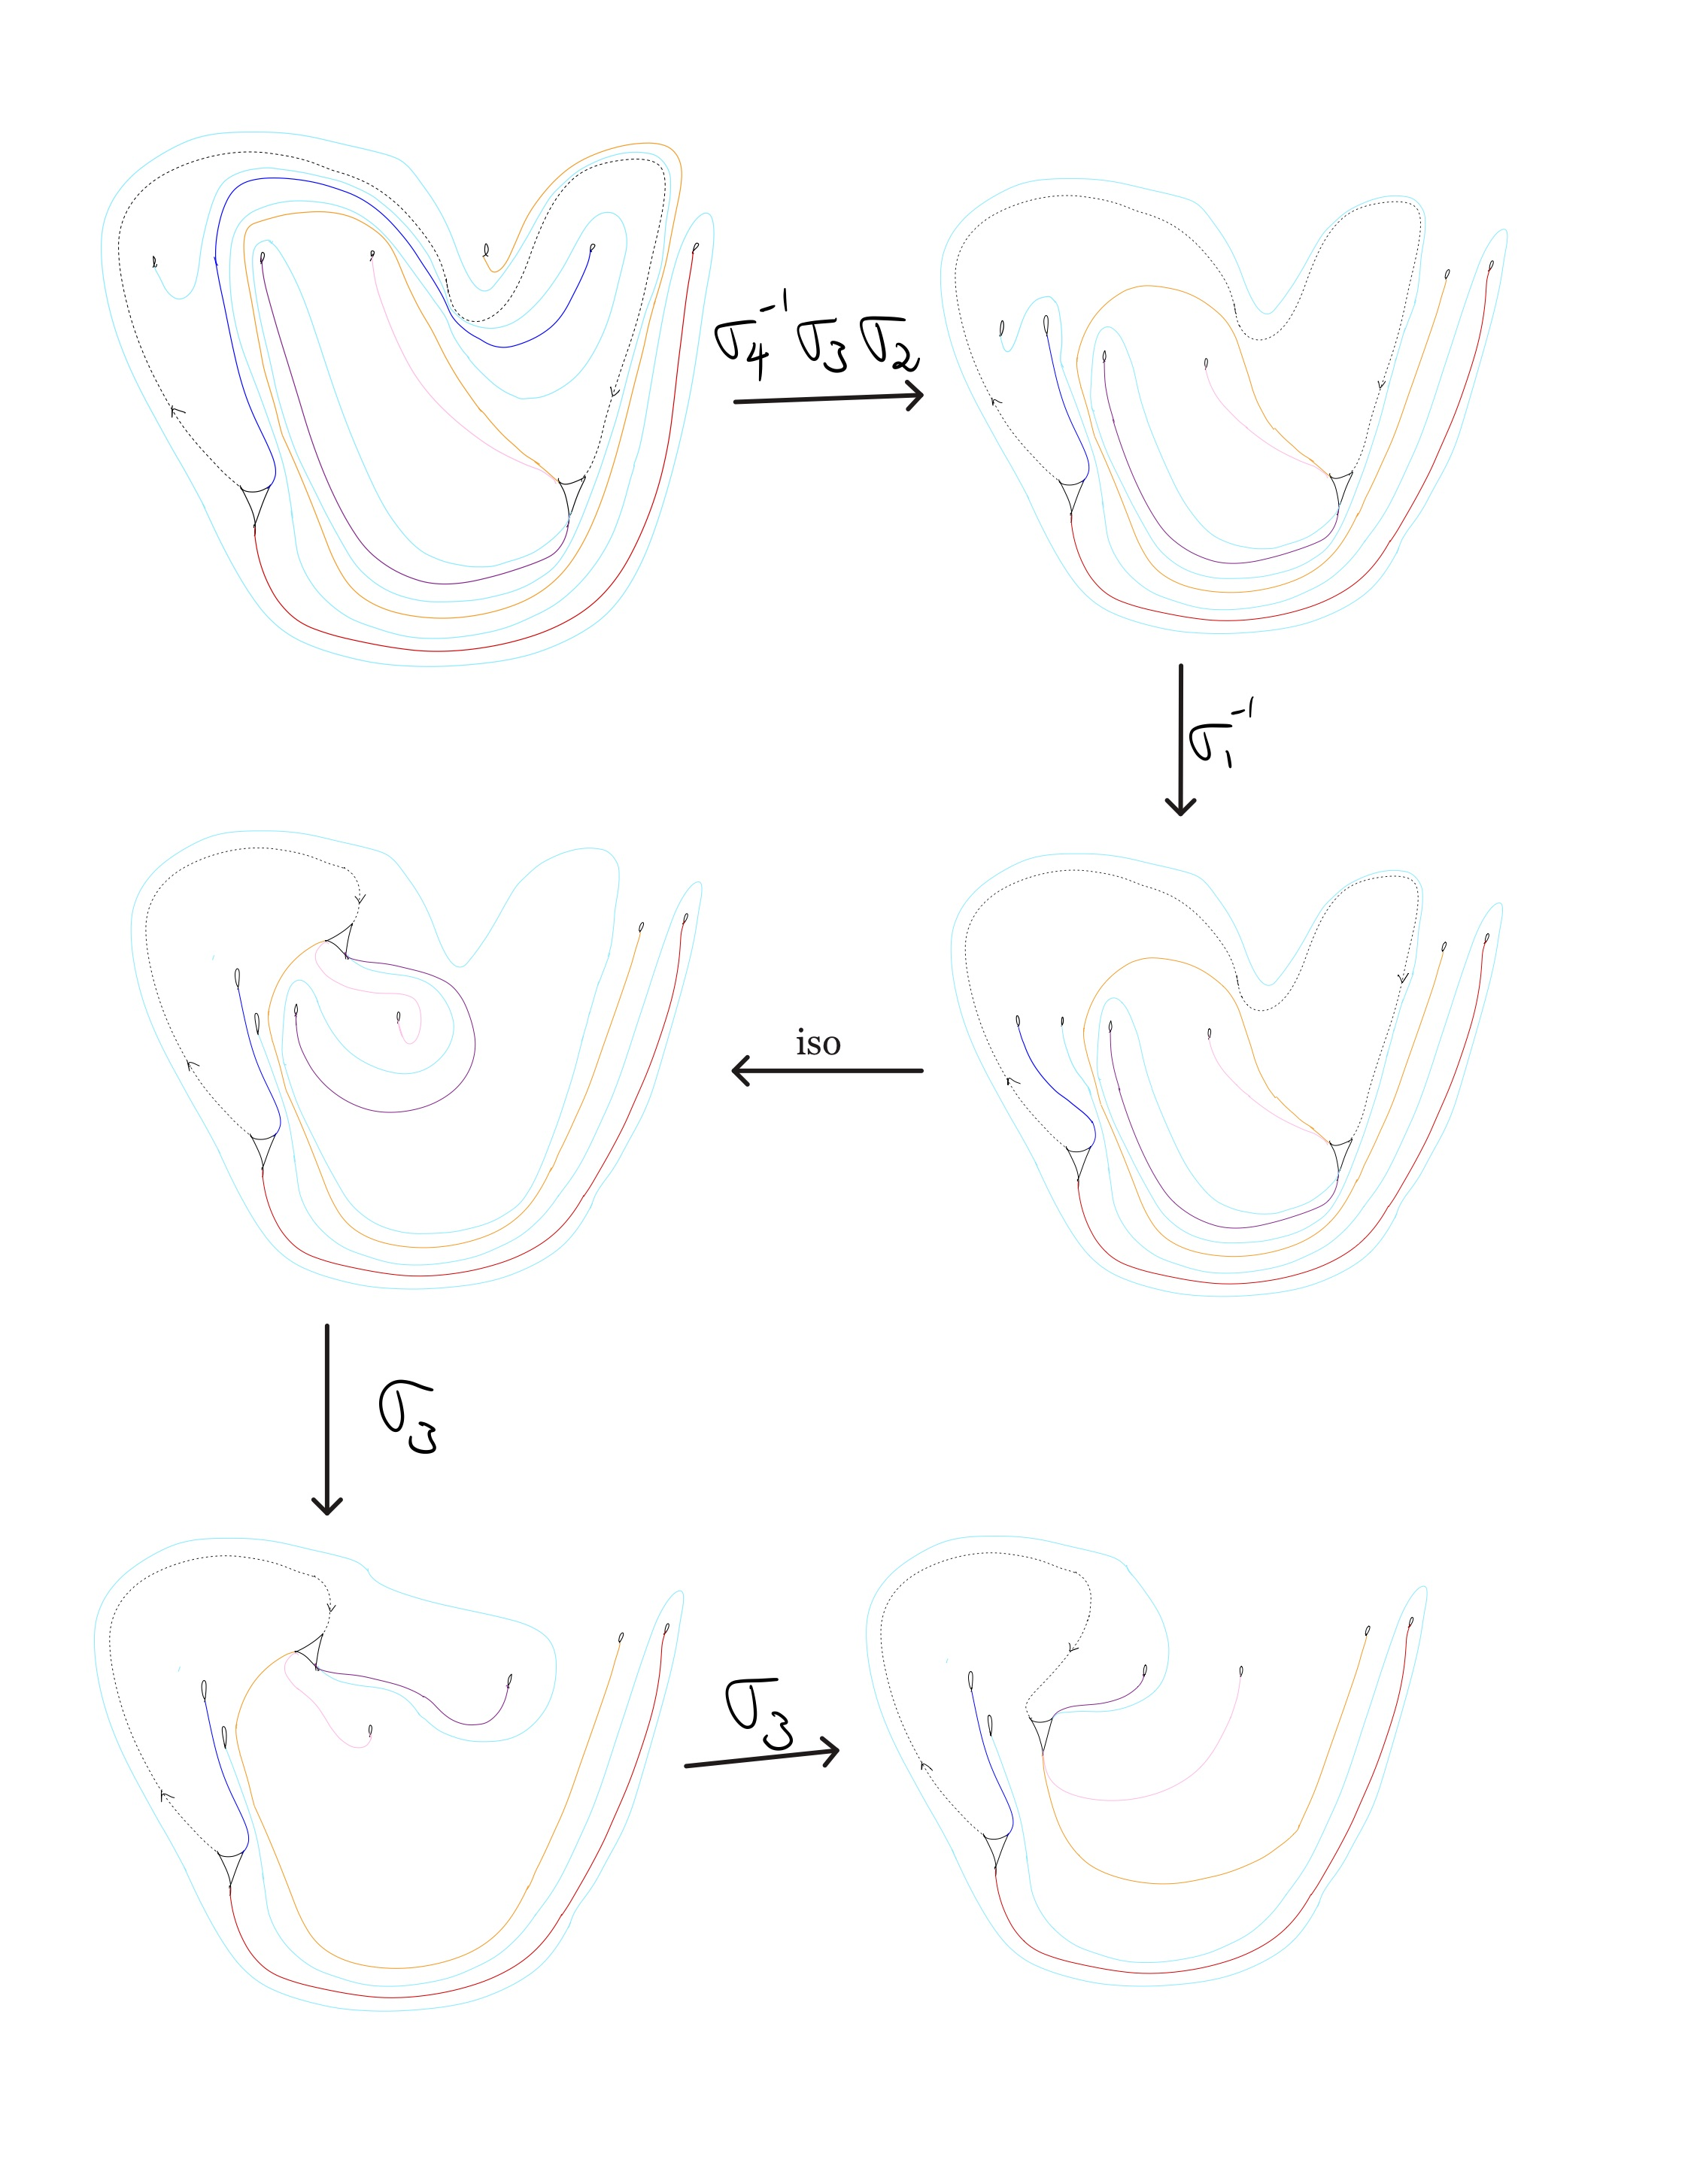
\includegraphics[width=\linewidth, height=0.45\textheight, keepaspectratio]{figures_braid/figures_track_13/Track 13 Braid 3 Boofus-2.jpg}%
    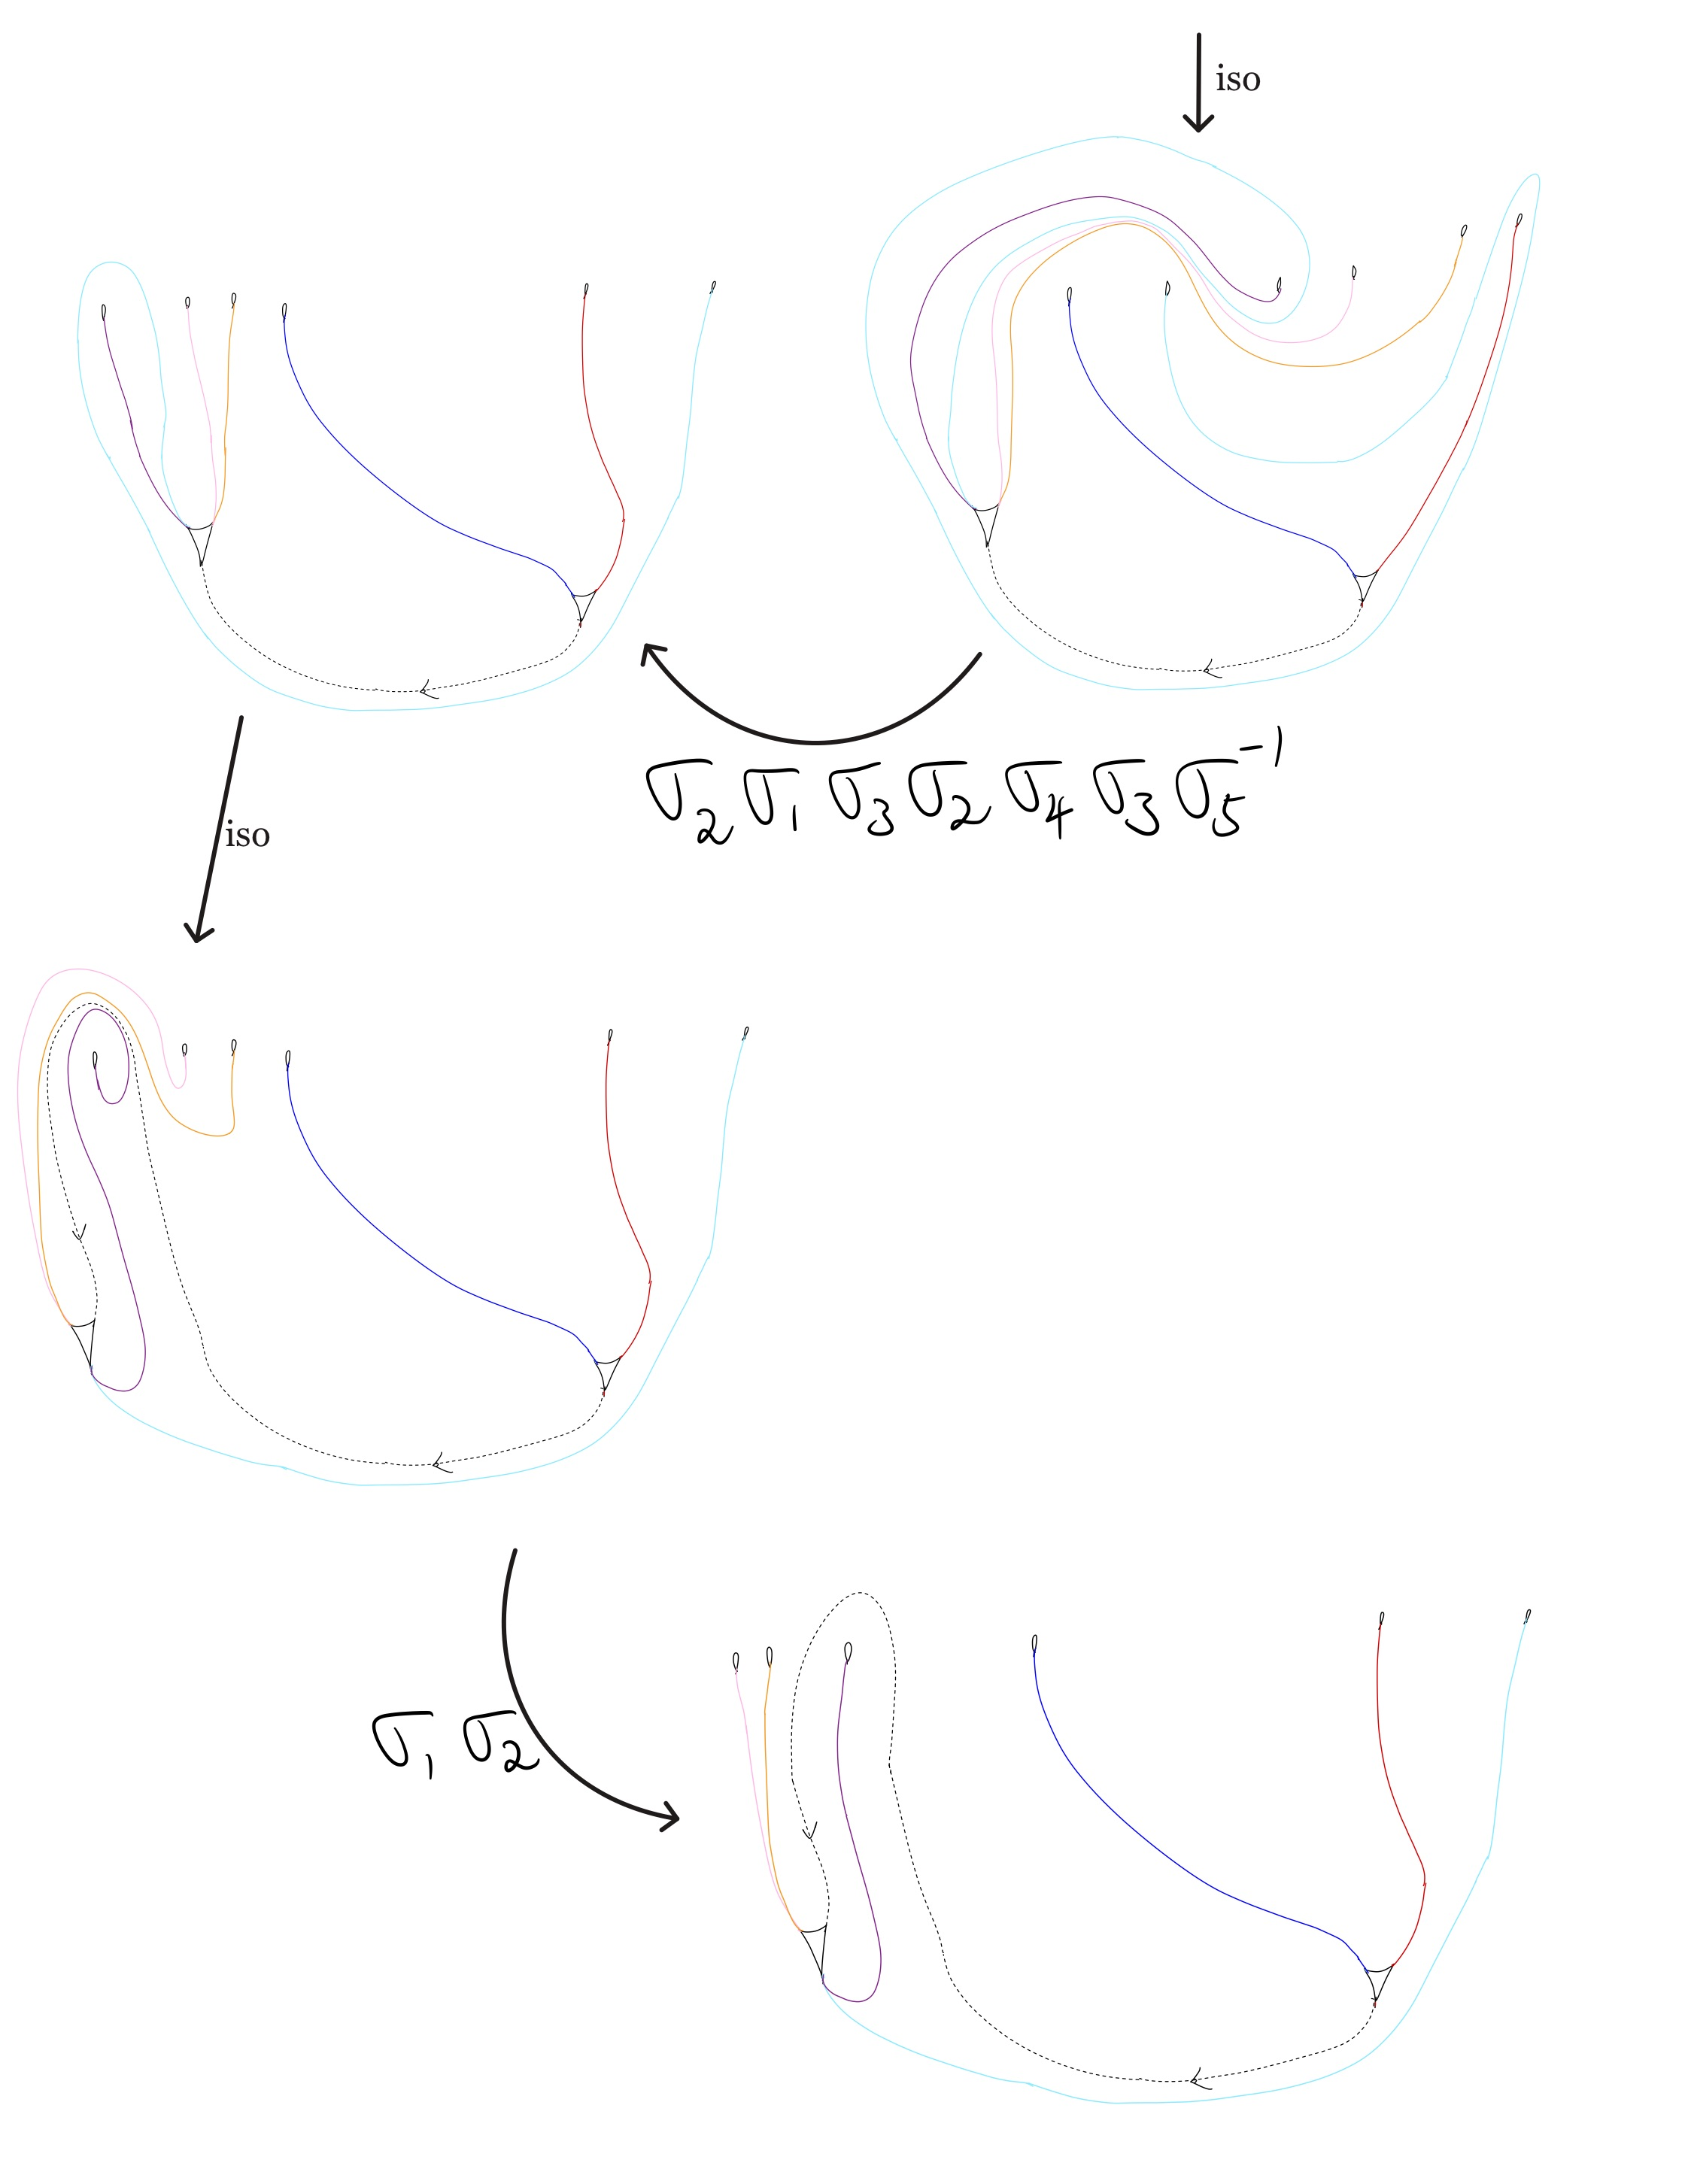
\includegraphics[width=\linewidth, height=0.45\textheight, keepaspectratio]{figures_braid/figures_track_13/Track 13 Braid 3 Boofus-3.jpg}
    \caption{This sequence shows the inverse of the braid $b_3^{13}$ carries Train Track Candidate Family 3.}
    \label{fig:track13_braid_b13_3}
\end{figure*}

\clearpage

\section{Candidate Family 4 (SCC)}\label{sec:track13_scc}
Train Track Map Candidate Family 4 of Track 13 is shown in Figure \ref{fig:track13_braid_b13_4_map}. See \ref{SCC} for details.

\begin{figure*}[ht]
    \centering
    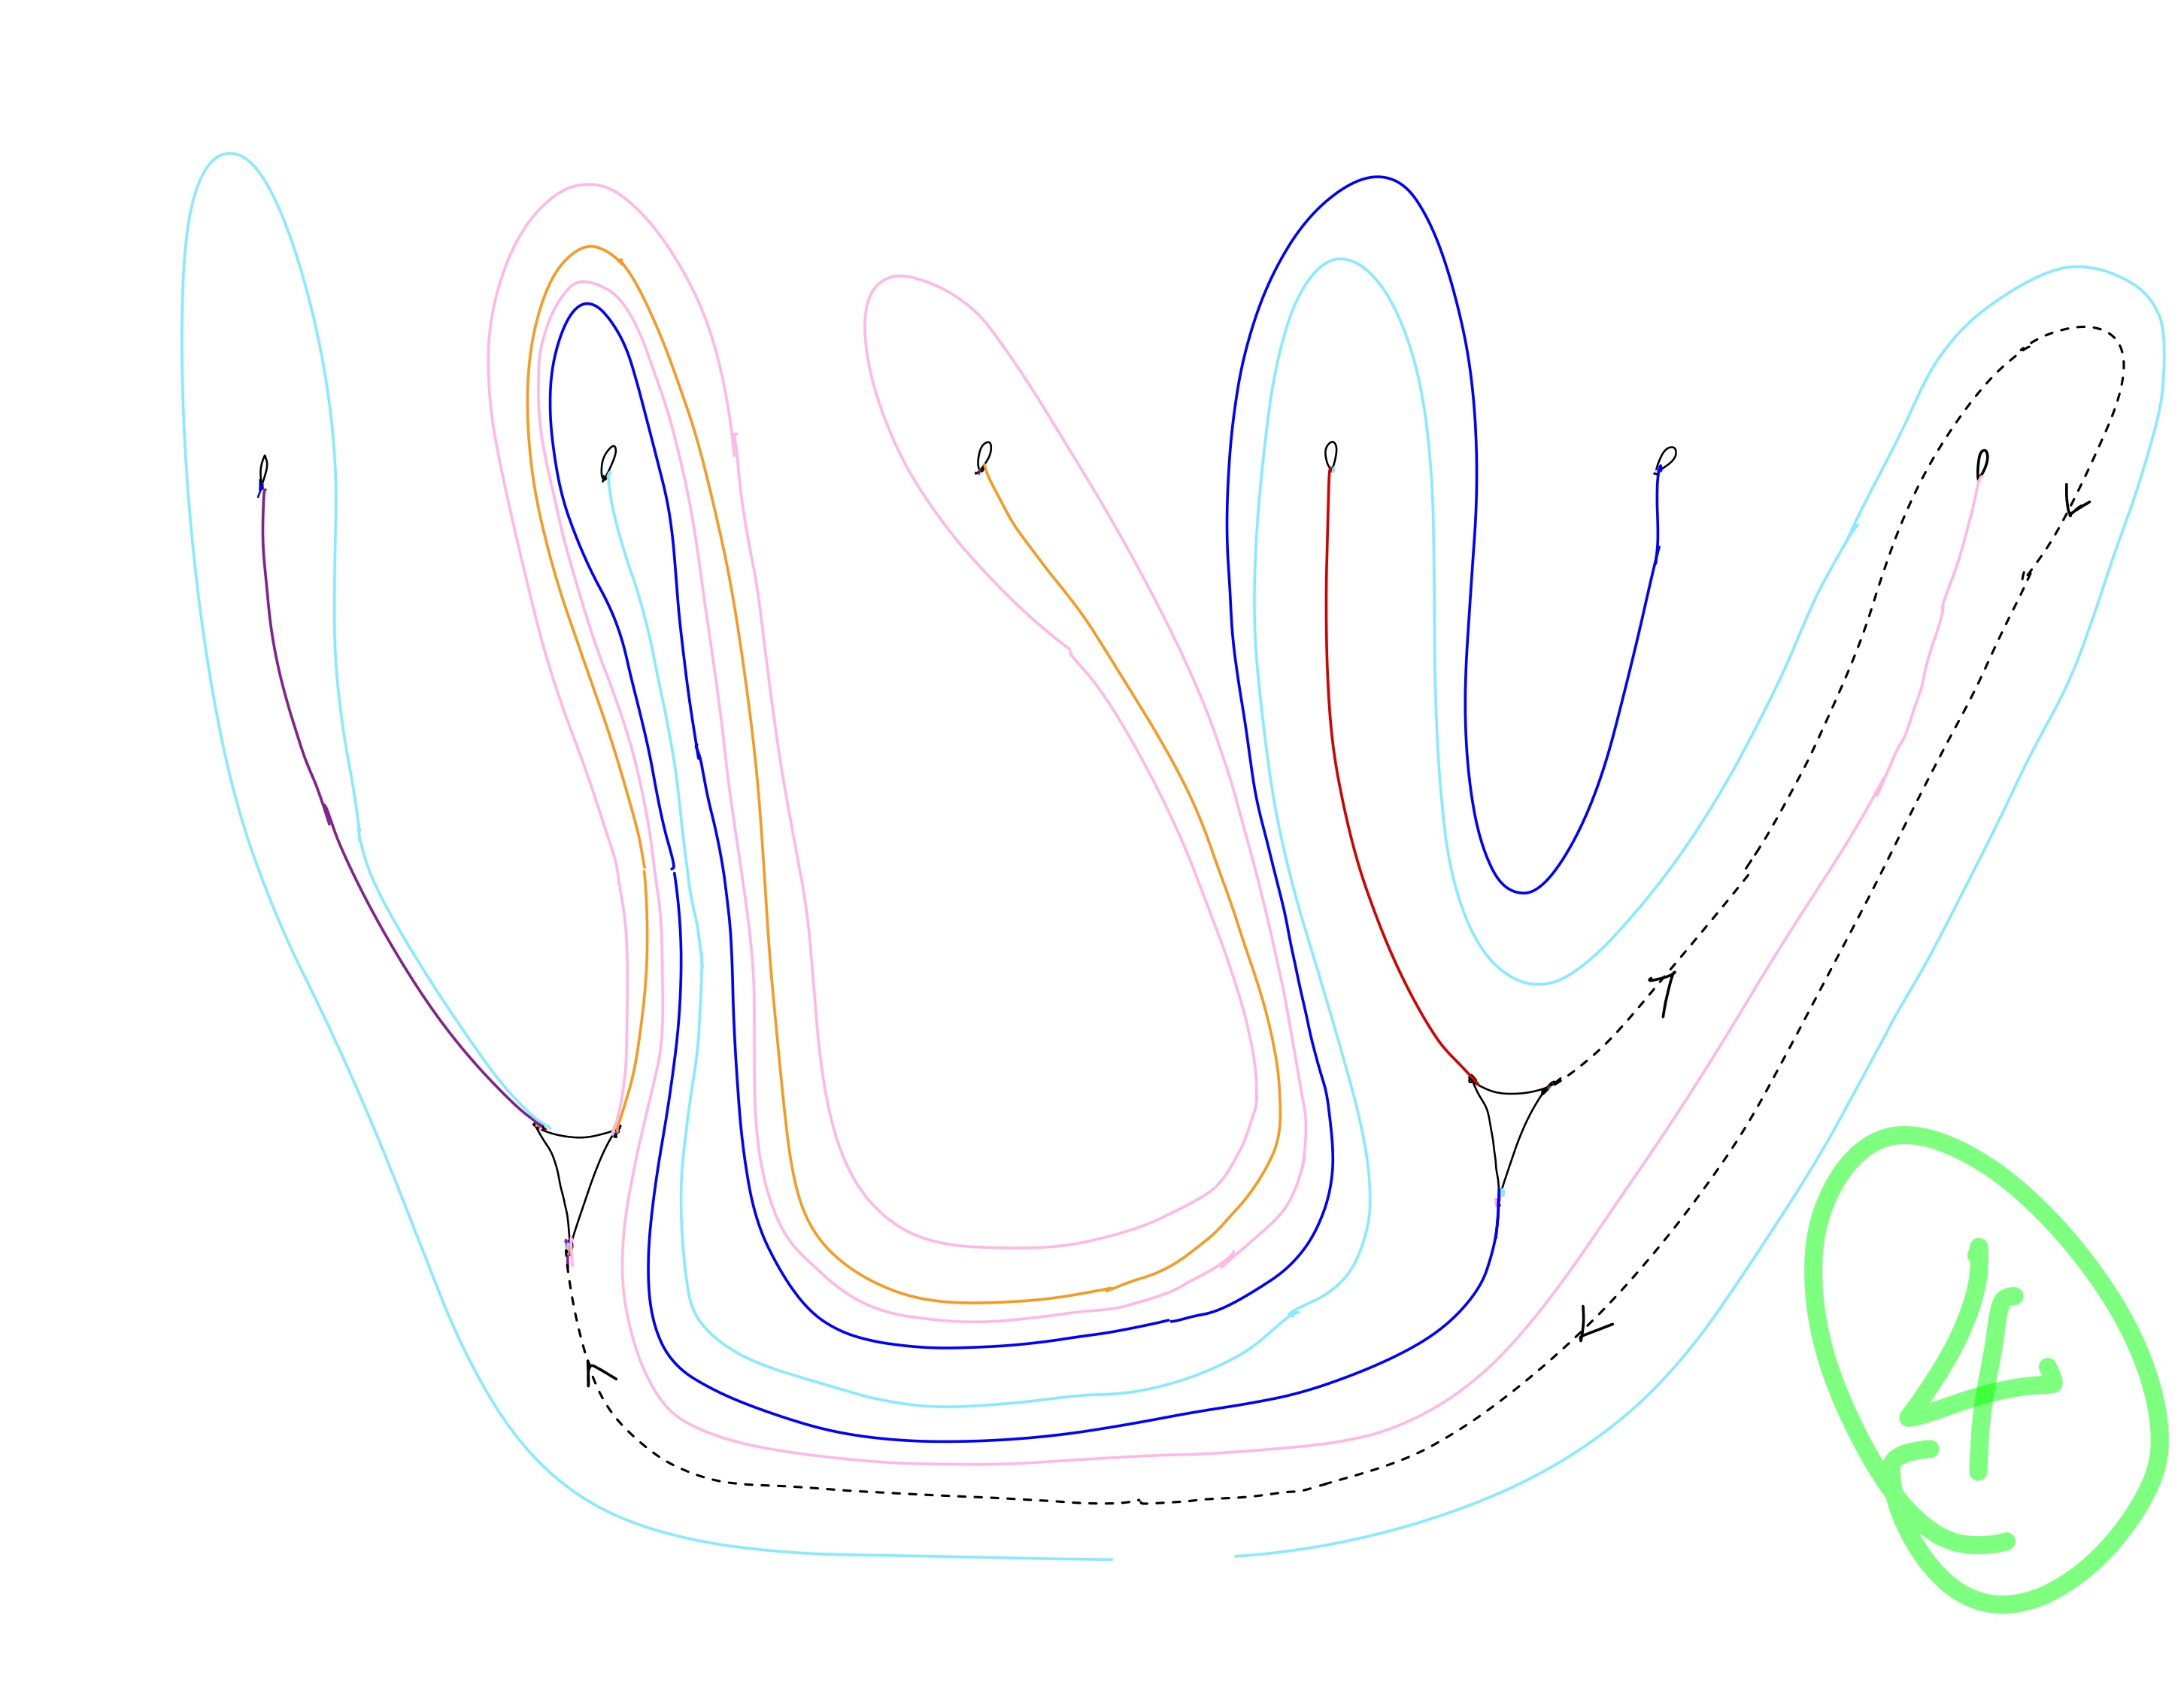
\includegraphics[width=\linewidth, height=0.45\textheight, keepaspectratio]{figures_braid/figures_track_13/Track 13 Braid 4 SCC-1.jpg}
    \caption{Train Track Map Candidate Family 4 (SCC) of Track 13.}
    \label{fig:track13_braid_b13_4_map}
\end{figure*}

The inverse of the following braid carries this family of train track maps:
\[
b_4^{13} = \sigma_{4} \sigma_{2} \sigma_{3} \sigma_{4}^{-1} \sigma_{5}^{-1} \sigma_{4}^{-1} \sigma_{5}^{-1} \sigma_{3}^{-1} \sigma_{4}^{-1} \sigma_{2} \sigma_{3}^{-1} \sigma_{2}^{-1} \sigma_{1}^{-1} \sigma_{1}^{-1} \circ L \circ \Lambda_6
\]

This is shown in Figure \ref{fig:track13_braid_b13_4}.

\begin{figure*}[p]
    \centering
    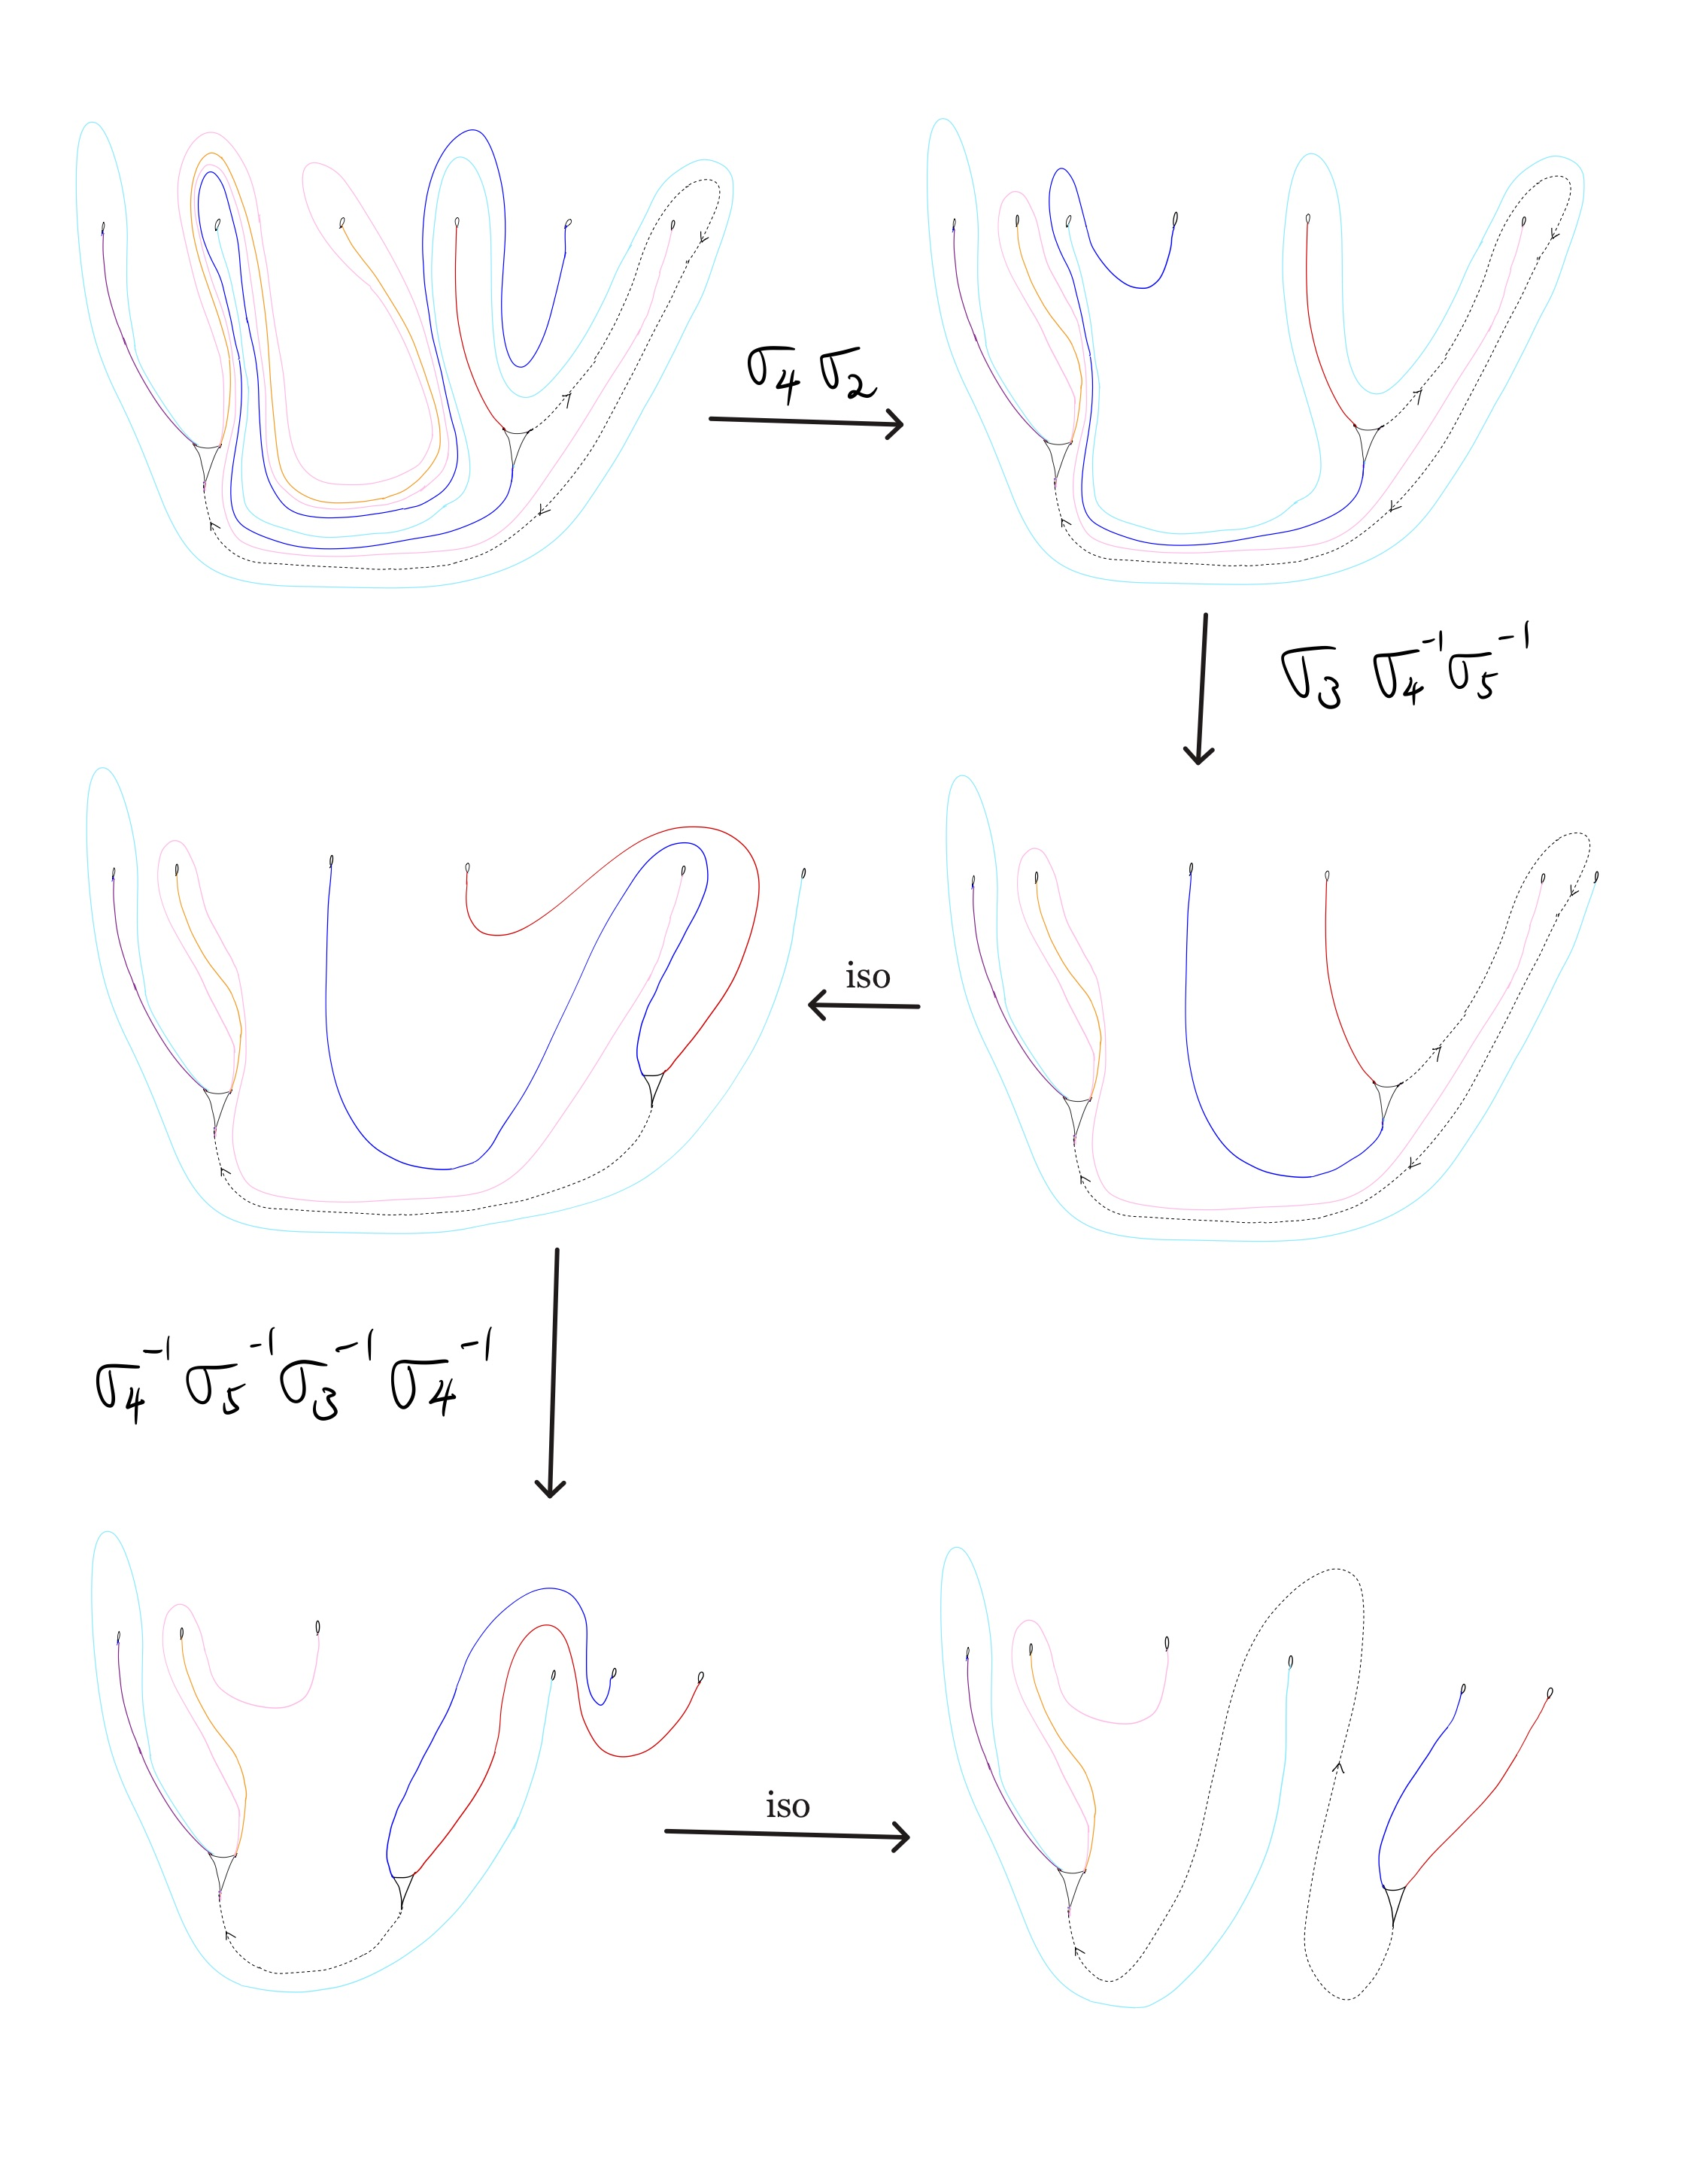
\includegraphics[width=\linewidth, height=0.45\textheight, keepaspectratio]{figures_braid/figures_track_13/Track 13 Braid 4 SCC-2.jpg}%
    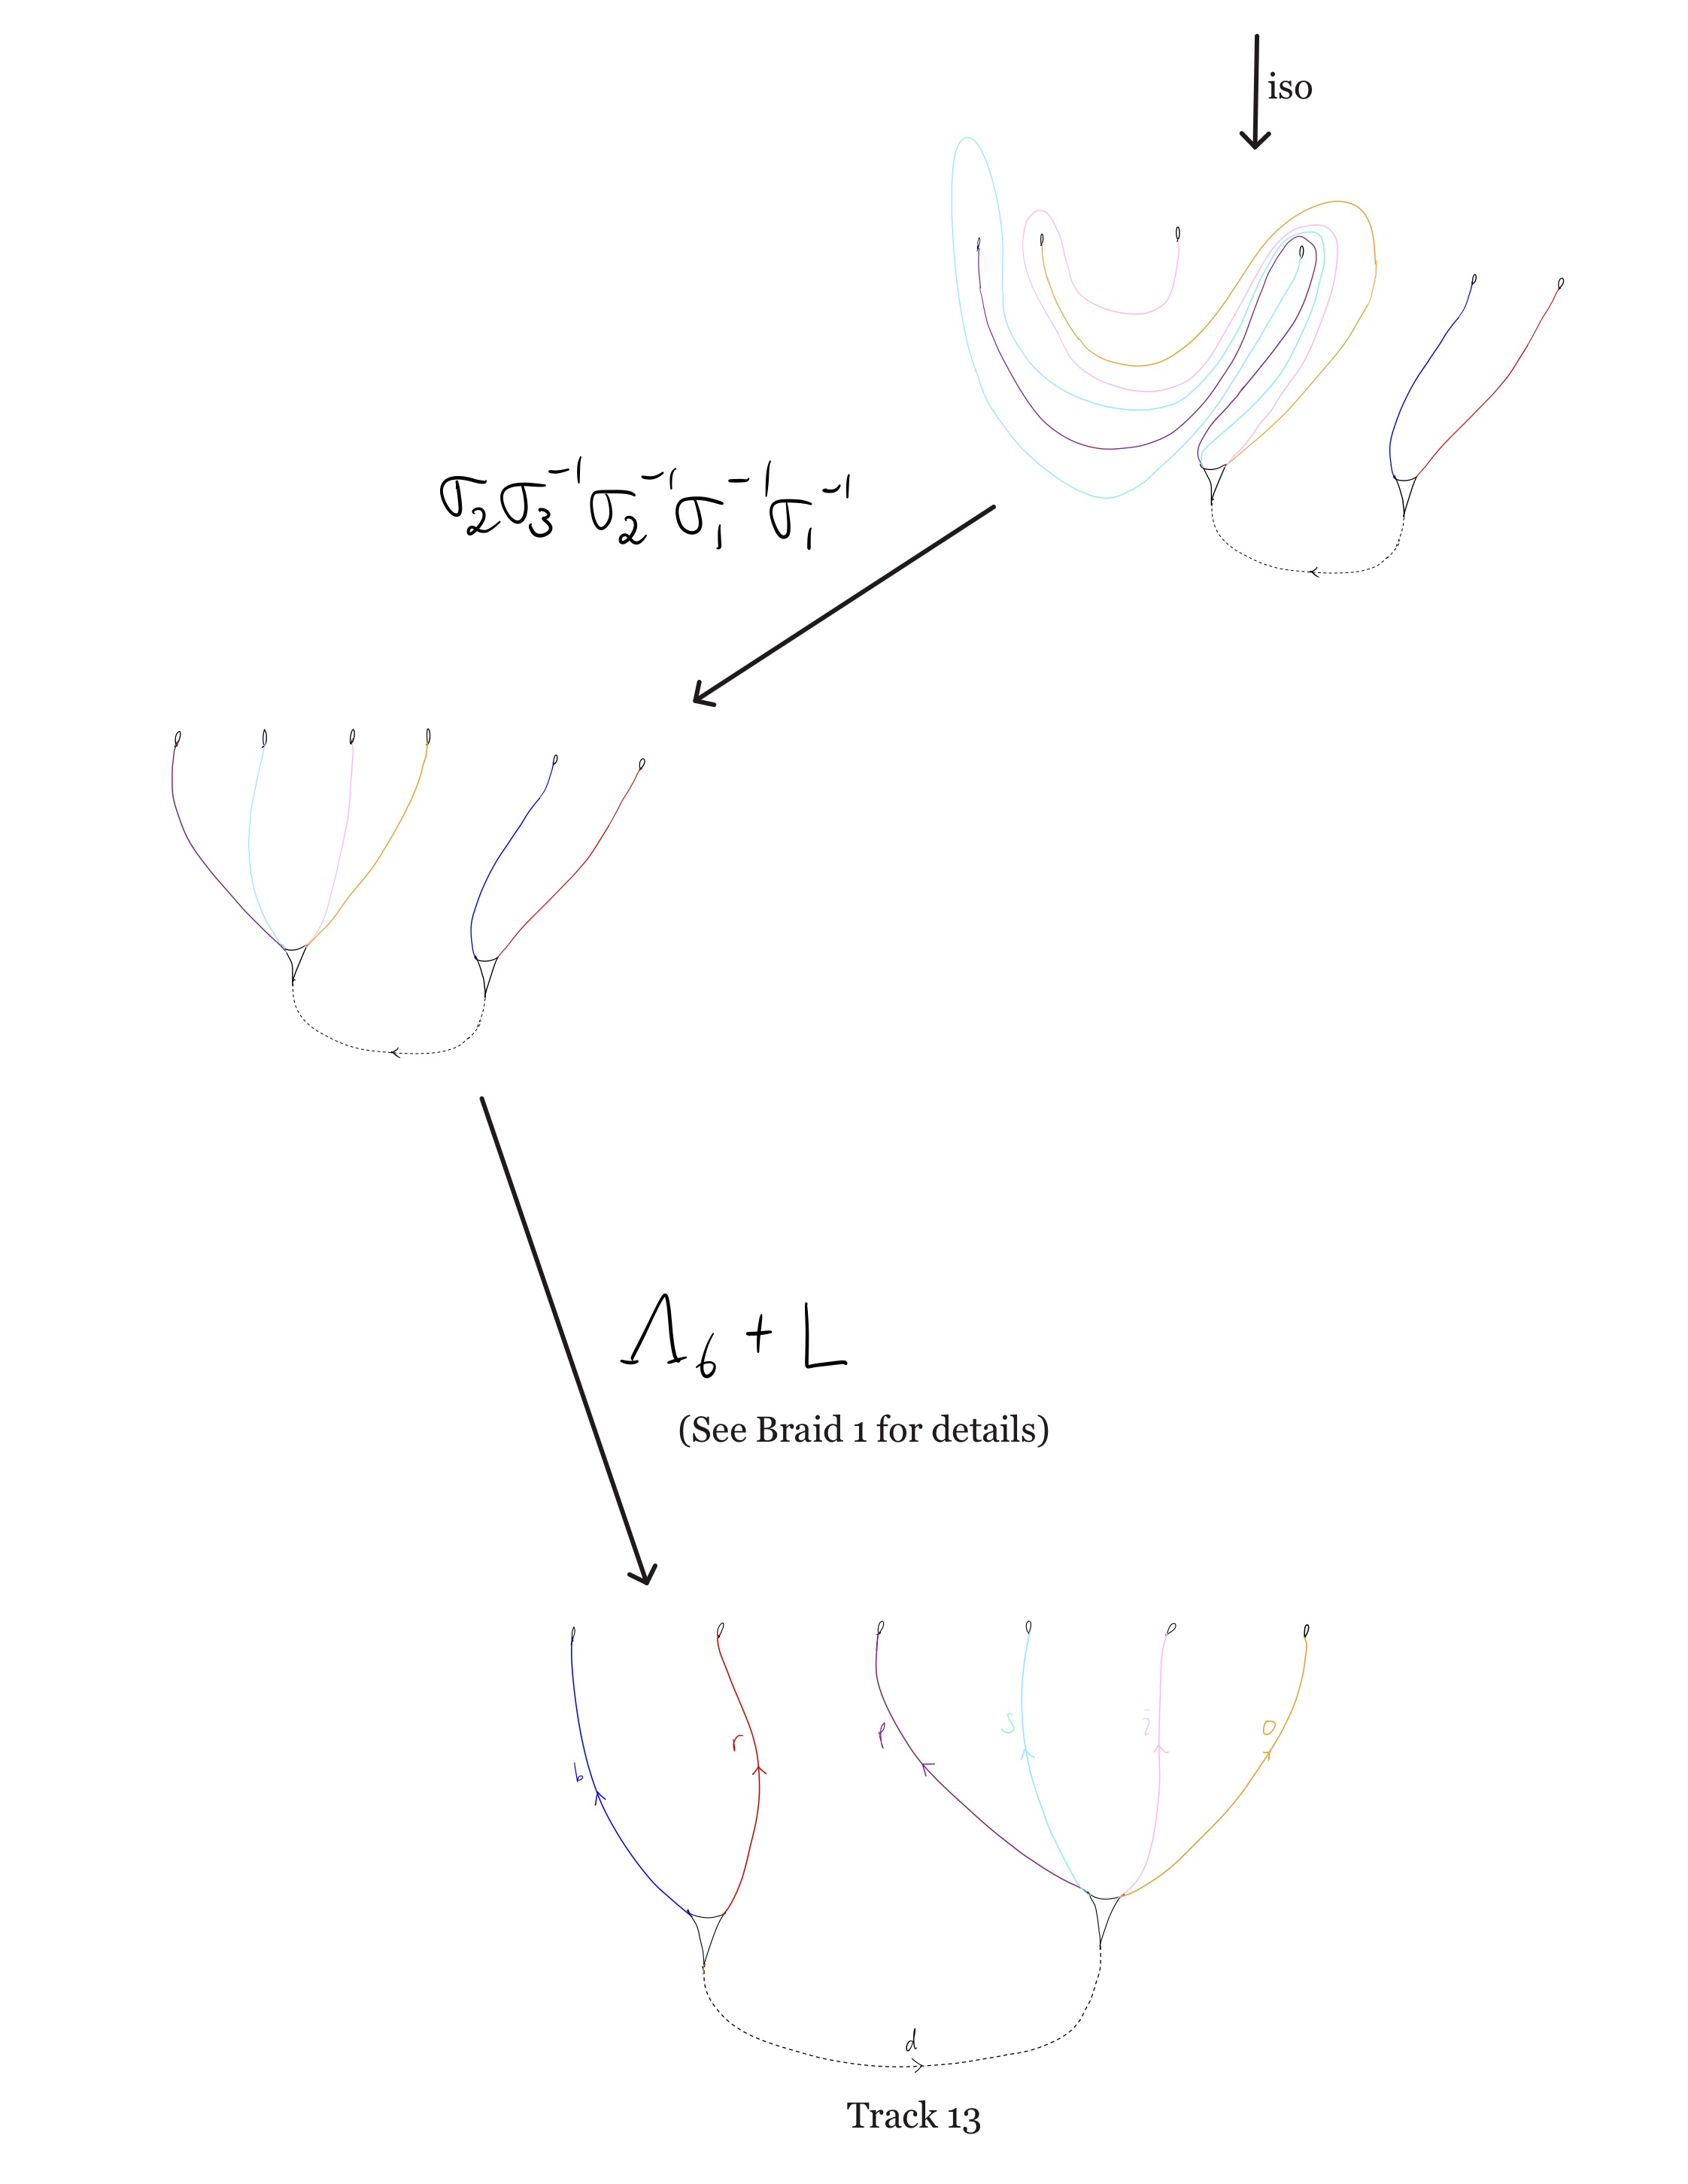
\includegraphics[width=\linewidth, height=0.45\textheight, keepaspectratio]{figures_braid/figures_track_13/Track 13 Braid 4 SCC-3.jpg}
    \caption{This sequence shows the inverse of the braid $b_4^{13}$ carries Train Track Candidate Family 4.}
    \label{fig:track13_braid_b13_4}
\end{figure*}

\clearpage